% Options for packages loaded elsewhere
\PassOptionsToPackage{unicode}{hyperref}
\PassOptionsToPackage{hyphens}{url}
%
\documentclass[
  man,floatsintext]{apa6}
\usepackage{amsmath,amssymb}
\usepackage{lmodern}
\usepackage{iftex}
\ifPDFTeX
  \usepackage[T1]{fontenc}
  \usepackage[utf8]{inputenc}
  \usepackage{textcomp} % provide euro and other symbols
\else % if luatex or xetex
  \usepackage{unicode-math}
  \defaultfontfeatures{Scale=MatchLowercase}
  \defaultfontfeatures[\rmfamily]{Ligatures=TeX,Scale=1}
\fi
% Use upquote if available, for straight quotes in verbatim environments
\IfFileExists{upquote.sty}{\usepackage{upquote}}{}
\IfFileExists{microtype.sty}{% use microtype if available
  \usepackage[]{microtype}
  \UseMicrotypeSet[protrusion]{basicmath} % disable protrusion for tt fonts
}{}
\makeatletter
\@ifundefined{KOMAClassName}{% if non-KOMA class
  \IfFileExists{parskip.sty}{%
    \usepackage{parskip}
  }{% else
    \setlength{\parindent}{0pt}
    \setlength{\parskip}{6pt plus 2pt minus 1pt}}
}{% if KOMA class
  \KOMAoptions{parskip=half}}
\makeatother
\usepackage{xcolor}
\usepackage{longtable,booktabs,array}
\usepackage{calc} % for calculating minipage widths
% Correct order of tables after \paragraph or \subparagraph
\usepackage{etoolbox}
\makeatletter
\patchcmd\longtable{\par}{\if@noskipsec\mbox{}\fi\par}{}{}
\makeatother
% Allow footnotes in longtable head/foot
\IfFileExists{footnotehyper.sty}{\usepackage{footnotehyper}}{\usepackage{footnote}}
\makesavenoteenv{longtable}
\usepackage{graphicx}
\makeatletter
\def\maxwidth{\ifdim\Gin@nat@width>\linewidth\linewidth\else\Gin@nat@width\fi}
\def\maxheight{\ifdim\Gin@nat@height>\textheight\textheight\else\Gin@nat@height\fi}
\makeatother
% Scale images if necessary, so that they will not overflow the page
% margins by default, and it is still possible to overwrite the defaults
% using explicit options in \includegraphics[width, height, ...]{}
\setkeys{Gin}{width=\maxwidth,height=\maxheight,keepaspectratio}
% Set default figure placement to htbp
\makeatletter
\def\fps@figure{htbp}
\makeatother
\setlength{\emergencystretch}{3em} % prevent overfull lines
\providecommand{\tightlist}{%
  \setlength{\itemsep}{0pt}\setlength{\parskip}{0pt}}
\setcounter{secnumdepth}{-\maxdimen} % remove section numbering
% Make \paragraph and \subparagraph free-standing
\ifx\paragraph\undefined\else
  \let\oldparagraph\paragraph
  \renewcommand{\paragraph}[1]{\oldparagraph{#1}\mbox{}}
\fi
\ifx\subparagraph\undefined\else
  \let\oldsubparagraph\subparagraph
  \renewcommand{\subparagraph}[1]{\oldsubparagraph{#1}\mbox{}}
\fi
\newlength{\cslhangindent}
\setlength{\cslhangindent}{1.5em}
\newlength{\csllabelwidth}
\setlength{\csllabelwidth}{3em}
\newlength{\cslentryspacingunit} % times entry-spacing
\setlength{\cslentryspacingunit}{\parskip}
\newenvironment{CSLReferences}[2] % #1 hanging-ident, #2 entry spacing
 {% don't indent paragraphs
  \setlength{\parindent}{0pt}
  % turn on hanging indent if param 1 is 1
  \ifodd #1
  \let\oldpar\par
  \def\par{\hangindent=\cslhangindent\oldpar}
  \fi
  % set entry spacing
  \setlength{\parskip}{#2\cslentryspacingunit}
 }%
 {}
\usepackage{calc}
\newcommand{\CSLBlock}[1]{#1\hfill\break}
\newcommand{\CSLLeftMargin}[1]{\parbox[t]{\csllabelwidth}{#1}}
\newcommand{\CSLRightInline}[1]{\parbox[t]{\linewidth - \csllabelwidth}{#1}\break}
\newcommand{\CSLIndent}[1]{\hspace{\cslhangindent}#1}
\ifLuaTeX
\usepackage[bidi=basic]{babel}
\else
\usepackage[bidi=default]{babel}
\fi
\babelprovide[main,import]{english}
% get rid of language-specific shorthands (see #6817):
\let\LanguageShortHands\languageshorthands
\def\languageshorthands#1{}
% Manuscript styling
\usepackage{upgreek}
\captionsetup{font=singlespacing,justification=justified}

% Table formatting
\usepackage{longtable}
\usepackage{lscape}
% \usepackage[counterclockwise]{rotating}   % Landscape page setup for large tables
\usepackage{multirow}		% Table styling
\usepackage{tabularx}		% Control Column width
\usepackage[flushleft]{threeparttable}	% Allows for three part tables with a specified notes section
\usepackage{threeparttablex}            % Lets threeparttable work with longtable

% Create new environments so endfloat can handle them
% \newenvironment{ltable}
%   {\begin{landscape}\centering\begin{threeparttable}}
%   {\end{threeparttable}\end{landscape}}
\newenvironment{lltable}{\begin{landscape}\centering\begin{ThreePartTable}}{\end{ThreePartTable}\end{landscape}}

% Enables adjusting longtable caption width to table width
% Solution found at http://golatex.de/longtable-mit-caption-so-breit-wie-die-tabelle-t15767.html
\makeatletter
\newcommand\LastLTentrywidth{1em}
\newlength\longtablewidth
\setlength{\longtablewidth}{1in}
\newcommand{\getlongtablewidth}{\begingroup \ifcsname LT@\roman{LT@tables}\endcsname \global\longtablewidth=0pt \renewcommand{\LT@entry}[2]{\global\advance\longtablewidth by ##2\relax\gdef\LastLTentrywidth{##2}}\@nameuse{LT@\roman{LT@tables}} \fi \endgroup}

% \setlength{\parindent}{0.5in}
% \setlength{\parskip}{0pt plus 0pt minus 0pt}

% Overwrite redefinition of paragraph and subparagraph by the default LaTeX template
% See https://github.com/crsh/papaja/issues/292
\makeatletter
\renewcommand{\paragraph}{\@startsection{paragraph}{4}{\parindent}%
  {0\baselineskip \@plus 0.2ex \@minus 0.2ex}%
  {-1em}%
  {\normalfont\normalsize\bfseries\itshape\typesectitle}}

\renewcommand{\subparagraph}[1]{\@startsection{subparagraph}{5}{1em}%
  {0\baselineskip \@plus 0.2ex \@minus 0.2ex}%
  {-\z@\relax}%
  {\normalfont\normalsize\itshape\hspace{\parindent}{#1}\textit{\addperi}}{\relax}}
\makeatother

% \usepackage{etoolbox}
\makeatletter
\patchcmd{\HyOrg@maketitle}
  {\section{\normalfont\normalsize\abstractname}}
  {\section*{\normalfont\normalsize\abstractname}}
  {}{\typeout{Failed to patch abstract.}}
\patchcmd{\HyOrg@maketitle}
  {\section{\protect\normalfont{\@title}}}
  {\section*{\protect\normalfont{\@title}}}
  {}{\typeout{Failed to patch title.}}
\makeatother

\usepackage{xpatch}
\makeatletter
\xapptocmd\appendix
  {\xapptocmd\section
    {\addcontentsline{toc}{section}{\appendixname\ifoneappendix\else~\theappendix\fi\\: #1}}
    {}{\InnerPatchFailed}%
  }
{}{\PatchFailed}
\keywords{replication value, replication, social neuroscience, bibliometric analysis, expected utility, exploratory report\newline\indent Word count: 9209}
\usepackage{csquotes}
\usepackage{caption}
\captionsetup[figure]{labelformat=empty}
\captionsetup[table]{labelformat=empty}
\usepackage{fancyhdr}
\pagestyle{fancy}
\lhead{ISAGER ET AL.}
\rhead{}
\ifLuaTeX
  \usepackage{selnolig}  % disable illegal ligatures
\fi
\IfFileExists{bookmark.sty}{\usepackage{bookmark}}{\usepackage{hyperref}}
\IfFileExists{xurl.sty}{\usepackage{xurl}}{} % add URL line breaks if available
\urlstyle{same} % disable monospaced font for URLs
\hypersetup{
  pdftitle={Selecting Studies for Replication in Social Neuroscience: Exploring a Formal Approach},
  pdfauthor={Peder Mortvedt Isager1, Daniël Lakens2, Thed van Leeuwen3, \& Anna E. van 't Veer4},
  pdflang={en-EN},
  pdfkeywords={replication value, replication, social neuroscience, bibliometric analysis, expected utility, exploratory report},
  hidelinks,
  pdfcreator={LaTeX via pandoc}}

\title{Selecting Studies for Replication in Social Neuroscience: Exploring a Formal Approach}
\author{Peder Mortvedt Isager\textsuperscript{1}, Daniël Lakens\textsuperscript{2}, Thed van Leeuwen\textsuperscript{3}, \& Anna E. van 't Veer\textsuperscript{4}}
\date{}


\shorttitle{Selecting Studies for Replication in Social Neuroscience}

\authornote{

This work was funded by VIDI grant 452-17-013. We want to thank all student assistants from Leiden University and Eindhoven University of Technology who contributed to data collection for this project at one point or another. All data to reproduce this manuscript can be found at \url{https://github.com/pederisager/NeuroRep_RV}.

The authors made the following contributions. Peder Mortvedt Isager: Conceptualization, Investigation, Visualization, Writing - Original Draft, Writing - Review \& Editing; Daniël Lakens: Funding acquisition, Supervision, Writing - Review \& Editing; Thed van Leeuwen: Data curation, Investigation, Resources; Anna E. van 't Veer: Conceptualization, Supervision, Investigation, Writing - Review \& Editing.

Correspondence concerning this article should be addressed to Anna E. van 't Veer, Wassenaarseweg 52, 2333 AK Leiden, Leiden University, Institute of Psychology, Methodology and Statistics unit.. E-mail: \href{mailto:a.e.van.t.veer@fsw.leidenuniv.nl}{\nolinkurl{a.e.van.t.veer@fsw.leidenuniv.nl}}

}

\affiliation{\vspace{0.5cm}\textsuperscript{1} Department of Psychology, Oslo New University College\\\textsuperscript{2} Department of Industrial Engineering \& Innovation Sciences, Eindhoven University of Technology\\\textsuperscript{3} Centre for Science and Technology Studies, Leiden University\\\textsuperscript{4} Methodology and Statistics unit, Institute of Psychology, Leiden University}

\abstract{%
Replication of published results is crucial for ensuring the robustness and self-correction of research, yet replications are scarce in many fields. Replicating researchers will therefore often have to decide which of several relevant candidates to target for replication. Formal strategies for efficient study selection have been proposed, but none have been explored for practical feasibility--a prerequisite for validation. Here we move one step closer to efficient replication study selection by exploring the feasibility of a particular selection strategy that estimates \emph{replication value} as a function of citation impact and sample size (Isager, Veer, \& Lakens, 2021) in the field of social neuroscience, where replication seems especially important. We first report our efforts to generate a representative candidate set of replication targets in social fMRI research. We then explore the feasibility and reliability of estimating replication value for the targets in our set, resulting in a dataset of 1358 studies ranked on their value of prioritising them for replication. In addition, we carefully examine possible measures, test auxiliary assumptions, and identify boundary conditions of measuring value and uncertainty. Our demonstrates the importance of how to implement study selection strategies in practice, and provides a general framework for exploring the feasibility of formal study selection strategies. We end our report by discussing how future validation studies might be designed.
}



\begin{document}
\maketitle

\hypertarget{introduction}{%
\section{Introduction}\label{introduction}}

Close replication of original research results is essential to increase our confidence that empirical findings are reliable (Schmidt, 2009). When a study procedure is repeated in a new sample (preferably by a novel research team), spurious data patterns generated by random chance, mistakes, fraud, or questionable research practices can be detected and discarded. Close replication reduces research waste by preventing researchers from building on seemingly promising findings that are not true. This is especially important in social and cognitive neuroscience. Research in these fields are often vulnerable to inflated false positive rates and overestimation of effect sizes due to a combination of (1) low statistical power (Szucs \& Ioannidis, 2017), (2) substantial researcher degrees of freedom that inflate the Type 1 error rate (Botvinik-Nezer et al., 2020; Carp, 2012), and (3) incentives to publish statistically significant results (Button et al., 2013). Unsurprisingly, rates of successful replications are low (Boekel et al., 2015). In spite of this, close replications of original studies are not common practice (Ashar et al., 2021; Huber, Potter, \& Huszar, 2019; Poldrack et al., 2017). At the same time, the cost of data collection in social neuroscience is high (Poldrack et al., 2017), which leads to a conundrum. On the one hand, high data collection costs make it all the more important to conduct close replications and prevent costly studies from being built on spurious findings. On the other hand, high costs limit how often replication studies can be conducted. With limited resources and many non-replicated studies to choose from, researchers in social and cognitive neuroscience should consider which studies in the published literature would be the most important to replicate, so that resources are directed towards replication can be spent optimally.

Various formal strategies for replication study selection have been developed in recent years (Field, Hoekstra, Bringmann, \& Van Ravenzwaaij, 2019; Isager et al., 2021; Matiasz et al., 2018; supplementary formula documents in \textbf{Isager2020?}). If effective, such strategies have great potential to increase the transparency and efficiency of replication study selection in neuroimaging research. When criteria for study selection are made transparent, it becomes easier to discuss which replication studies are most important to fund, conduct, and publish. Additionally, formal strategies allow researchers who agree on criteria to more easily identify and coordinate replication of high-value studies in their field. By increasing the efficiency of coordination and resource spending in replication research, formal study selection strategies present a major step forward towards the important goal of making replication part of mainstream research practice.

However, no formal study selection strategies have been tested for application in social neuroscience. To be applicable, a strategy must meet two basic conditions. First, it must be feasible to apply the strategy in practice. That is, the information needed to execute the strategy must be possible to obtain given reasonable time and resource constraints. Most formal study selection strategies are based on a combination of statistical, bibliometric, and substantive information about the candidate studies, which is often not easy to access (Federer et al., 2018; Furukawa, Barbui, Cipriani, Brambilla, \& Watanabe, 2006; Glasziou, Meats, Heneghan, \& Shepperd, 2008; Sullivan \& Feinn, 2012; e.g., Tay, Kramer, \& Waltman, 2020). The feasibility of existing strategies for application in any particular area of research is therefore uncertain. Second, provided that the strategy is feasible to apply we must validate that the strategy is actually helping us reach our prespecified research goals. All feasible selection strategies lead to \emph{some} prioritization of studies, but whether this prioritization has any validity and practical utility is an empirical question.

In this article we explore how feasible it is to apply a particular replication study selection strategy (Isager et al., 2021) to fMRI research in social neuroscience. We focus on fMRI research in social neuroscience because replication studies in this field are both scarce and costly, and because this is a field of expertise of the first and last author. We reflect on the generalizability of our conclusions to other research areas in the general discussion. Before we are ready to compare different study selection strategies that have been proposed, we believe it is important to lay the ground work for such a comparison. After conceptualizing citation count as an indicator of the value of a study, and sample size as an indicator of uncertainty (Isager et al., 2021) here we take the next step by examining the following elements that are required to make a future comparison of study selection strategies more meaningful, based on Scheel, Tiokhin, Isager, and Lakens (2021). First, we explore different measures of citation impact, and examine if the source of the citation information matters for the rank-order of targets to select for replication. Second, we empirically examine the relationship between different ways that the value and impact of studies can be operationalized by their citation count and sample size. Third, we identify examples of boundary conditions where the value of a study and the uncertainty about a study are not captured by the citation count and sample size, based on an in-depth evaluation process of a subset of replication candidates. Finally, we examine three auxiliary assumptions regarding 1) the possibility to control for the age of the article when computing the replication value based on the citation count, 2) that the source of the citation counts does not substantially impact the rank-order, and 3) that past citation counts predict future citation counts.

We perform these four steps through a feasibility study, where we also examine if it is possible to code the required information to quantify uncertainty. We explore whether the steps of a study selection strategy can be carried out in practice given reasonable time- and resource constraints. We end with a brief qualitative assessment of the studies recommended to us by the strategy, noting potential issues that future validation studies should examine more carefully. The primary goal in this article is to understand how best to implement the strategy of (Isager et al., 2021) in social fMRI research so that the strategy can be validated for use in this field and potentially used for efficient study selection by future researchers. A secondary goal of this article is to curate a comprehensive set of empirical studies in the social fMRI literature that could form the basis for any replication study selection in this field, regardless of the selection strategy utilized. We summarize information about this set of studies, such as their citation counts and sample sizes, descriptively. By exploring information relevant to replication study selection in social fMRI we hope to leave researchers in this field better equipped to make well-informed decisions about which original research to prioritize for replication.

\hypertarget{a-four-step-approach-to-select-studies-for-replication}{%
\section{A four step approach to select studies for replication}\label{a-four-step-approach-to-select-studies-for-replication}}

To decide on a method for replication study selection, we must first settle on a goal, and a rationale for why selecting certain studies helps us reach this goal more efficiently. We use the formal decision model for replication study selection proposed by (\textbf{Isager2020?}). According to this model, the goal of a replication effort is to maximize the \emph{expected utility} of knowledge gained. \emph{Expected utility gain} can be approximated by the \emph{replication value} of the target claim we want to replicate. In this model replication value is a function of the \emph{value} (or importance) of having accurate knowledge about the target claim, and our \emph{uncertainty} about the truth status of the claim based on available evidence prior to replicating. Research claims that are highly valuable or important, and about which we are highly uncertain, will have a high replication value, and should be prioritized for replication in order to maximize expected utility gain.

We have previously proposed an operational definition of replication value (Isager et al., 2021), in which value is operationalized as the average yearly citation impact of the article in which a claim is reported, and uncertainty is operationalized as the sample size used to investigate the claim. Replication value is then operationalized as the indicator \emph{RV\textsubscript{Cn}}:

\begin{equation} 
  \tag{1}
  RV_{Cn} = value\times uncertainty = \frac{w(C_{S})}{Y+1}\times\frac{1}{\sqrt{n}}
  \label{eq:1}
\end{equation}

where \(RV_{Cn}\) denotes a particular operationalization of replication value, \(C\) stands for citation impact, \(n\) stands for the total number of participants included in the study, \(w()\) stands for the weighting function that should be applied to the citation impact (such as removing self-citations or not), \(s\) denotes the source the citation data is retrieved from, and \(Y\) stands for the age of the article in years. The equation assumes that average yearly citation impact is causally influenced by scientific impact, and that scientific impact partly determines the value of a claim. It also assumes that sample size partly determines the standard error of estimates in a study, which in turn partly determines the uncertainty about claims studied. Although both the average citation per year and the sample size are imperfect measures of value and uncertainty, our auxiliary assumption is that they are sufficiently correlated with value and uncertainty to generate a useful rank order of replication value.

We propose a four-step procedure for replication study selection based on \emph{RV\textsubscript{Cn}} (see Figure 1). In the first step an initial set of candidate studies is identified based on the research interests and resource constraints of the replicating researcher. As with every systematic review of the literature, the scope needs to be broad enough to encompass all claims of interest to the researchers, but narrow enough so that the review process remains feasible. In the second step \emph{RV\textsubscript{Cn}} is calculated for each study included in the set to create an initial estimate of rank-order expected utility gain. In the third step a subset of the studies with the highest \emph{RV\textsubscript{Cn}} is inspected in-depth by reading the article. This step functions as an additional check of the \emph{RV\textsubscript{Cn}} estimates, and has as the primary goal to evaluate additional factors relevant to the value and the uncertainty of the reported effect (e.g., Field et al., 2019; Heirene, 2021; KNAW, 2018). In this step researchers can also evaluate the feasibility of a replication study given the resources they have available, and the extent to which a replication study will be able to reduce uncertainty about the effect (\textbf{Isager2020?}). In the fourth step the candidate deemed most worthwhile to replicate is selected. Alternatively, if the researcher thinks the subset of studies that has been inspected contains no candidate that is worth replicating or feasible to replicate, step 3 and 4 can be repeated for a second subset of studies.

\begin{figure}
\centering
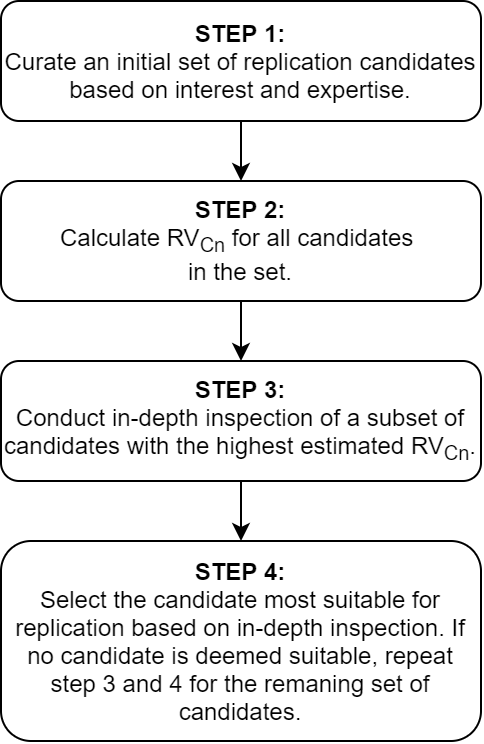
\includegraphics[width=0.5\textwidth,height=\textheight]{Figure_1.png}
\caption{\textbf{Figure 1.} General study selection procedure in which the \emph{RV\textsubscript{Cn}} indicator is implemented.}
\end{figure}

\hypertarget{exploring-the-feasibility-of-using-rvcn-for-study-selection-in-social-neuroscience}{%
\section{\texorpdfstring{Exploring the feasibility of using \emph{RV\textsubscript{Cn}} for study selection in Social Neuroscience}{Exploring the feasibility of using RVCn for study selection in Social Neuroscience}}\label{exploring-the-feasibility-of-using-rvcn-for-study-selection-in-social-neuroscience}}

\emph{RV\textsubscript{Cn}} was developed to enable a more efficient coordination of replication efforts. However, it is not clear whether it is feasible to use \emph{RV\textsubscript{Cn}} in practice for study selection in a research area such as social fMRI research. Our exploration focuses on the first two steps of the four-step procedure listed in Figure 1. We report the results of our attempt to implement these steps in practice, including our method for collecting a sample set of replication candidates (step 1), and more importantly, our method for collecting the citation impact and sample size data necessary to calculate \emph{RV\textsubscript{Cn}}, the reliability of our methods for generating accurate measures of citation counts and sample sizes, and describe the distribution of \emph{RV\textsubscript{Cn}} for our set of candidates (step 2). In supplementary materials we also summarize our unsuccessful pilot efforts to collect additional quantitative information related to the \emph{main finding} for each candidate studies in our set. Where a main finding could often be identified based on the abstract, it proved too difficult to identify which statistical test was the basis of this main finding. Finally, we also provide a brief qualitative evaluation of the recommendations produced by \emph{RV\textsubscript{Cn}} to better understand what sort of studies are being recommended, what the boundary conditions of this study selection strategy are, and to understand the factors one might want to evaluate in when implementing step 3. We conclude the article by generating hypotheses for studies that could be undertaken to test the validity of \emph{RV\textsubscript{Cn}}.

\hypertarget{step-1---determining-an-initial-set-of-candidate-studies}{%
\subsection{Step 1 - Determining an initial set of candidate studies}\label{step-1---determining-an-initial-set-of-candidate-studies}}

\hypertarget{eligibility-criteria}{%
\subsubsection{Eligibility criteria}\label{eligibility-criteria}}

To test the feasibility of calculating \emph{RV\textsubscript{Cn}} we first set out to determine a suitable set of candidate articles. This step is similar to any systematic literature review (e.g., a meta-analysis). We restricted our search for studies to fMRI research within social neuroscience between 2009-2019 at the time this decision was made. Although there is no need to restrict study selection to a specific time period, we reasoned that researchers might be especially interested in conducting replications of studies within a relatively recent time window to prevent unproductive follow-up research (when the original research is non-replicable) or stimulate follow-up research (when the original research is replicable).

\hypertarget{search-strategy}{%
\subsubsection{Search strategy}\label{search-strategy}}

We used the Web of Science (WoS; www.webofknowledge.com) database to construct our candidate dataset. WoS does not have a predefined field category for social neuroscience. To identify articles related to social neuroscience, we implemented a two-pronged search strategy on 2019-02-21. We first identified four journals in the WoS database as social neuroscience journals (Social Cognitive and Affective Neuroscience; Social Neuroscience; Behavioral Neuroscience; and Socioaffective Neuroscience Psychology). Empirical articles published in these journals were identified by submitting the following search term to Web of Science:

\begin{quote}
(SO=(social neuroscience OR social cognitive and affective neuroscience OR behavioral neuroscience OR socioaffective neuroscience psychology) AND PY=( 2019 OR 2009 OR 2018 OR 2017 OR 2016 OR 2015 OR 2014 OR 2013 OR 2012 OR 2011 OR 2010 )) AND DOCUMENT TYPES: (Article)
Timespan: 2009-2019. Indexes: SCI-EXPANDED, SSCI, A\&HCI, CPCI-S, CPCI-SSH, ESCI.
\end{quote}

To identify social neuroscience articles in general topic journals we searched the entire WoS database for articles containing the keywords ``social'' and ``fMRI'' in all fields. Empirical articles containing the relevant keyword information were identified by submitting the following search term to WoS:

\begin{quote}
ALL FIELDS: (fmri AND social)
Refined by: DOCUMENT TYPES: ( ARTICLE )
Timespan: 2009-2019. Indexes: SCI-EXPANDED, SSCI, A\&HCI, CPCI-S, CPCI-SSH, ESCI.
\end{quote}

2706 records were identified via this search strategy.

\hypertarget{selection-process}{%
\subsubsection{Selection process}\label{selection-process}}

The two search strategies yielded overlapping results. After removing duplicate records, the two search strategies yielded 7413 unique empirical articles in total (see Figure 2). Basic bibliometric information about each article, including author-provided keywords, were downloaded for all articles.

Authors PMI and AvtV reviewed the initial set of articles and excluded articles they did not believe would be feasible to replicate given their expertise and available resources, which meant excluding animal model research, highly invasive study designs, imaging methods outside our area of expertise, research on patient groups, and other keywords signaling the study would require highly specific samples, procedures, or technologies to perform. At this stage, exclusion criteria were not predetermined, but were exploratorily derived through inspecting keyword information in our initial candidate set. To ensure transparency a written record of the decision rationale for each excluded keyword has been made openly available on OSF (\url{https://osf.io/mtx72/}). Our final set of candidates contained 2268 empirical articles.

\begin{figure}
\centering
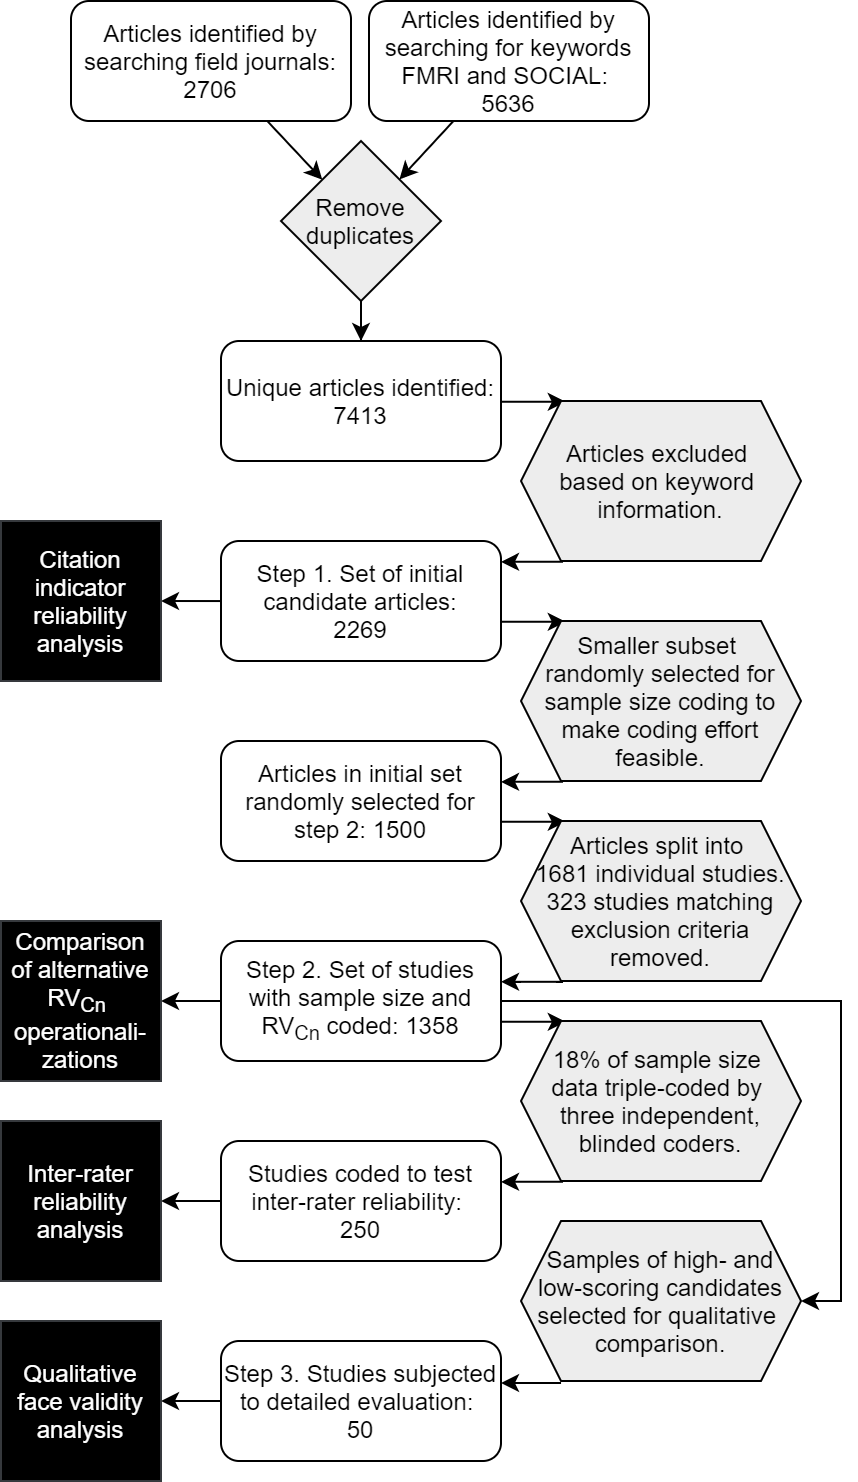
\includegraphics{sample_selection_process.png}
\caption{\textbf{Figure 2.} Overview of candidate selection process and data points available for each respective analysis reported below.}
\end{figure}

\hypertarget{exploration-of-sample-representativeness}{%
\subsubsection{Exploration of sample representativeness}\label{exploration-of-sample-representativeness}}

Once the final set of candidate records was determined, we explored the available bibliographic information to ensure that the sample indeed seemed representative of the field of social fMRI research. The full dataset, including all bibliometric variables and a variable codebook, are available on OSF (\url{https://osf.io/f7zdq/}). The articles included in our dataset were published in 329 unique journals, consistent with our expectation that social neuroscience is a broad and loosely connected discipline of researchers from many subfields, who publish in a variety of specialty- and general-topic journals. Table 1 displays the name and frequency of the 20 journals most frequently published in (70.99\% of all articles in the set were published in these 20 journals).

\begin{table}[tbp]

\begin{center}
\begin{threeparttable}

\caption{\label{tab:tab1}\textbf{Table 1:} Journals which the articles in our initial candidate set were most frequently published in.}

\begin{tabular}{ll}
\toprule
Journal & \multicolumn{1}{c}{Frequency}\\
\midrule
Social Cognitive And Affective Neuroscience & 324\\
Neuroimage & 236\\
Frontiers In Human Neuroscience & 115\\
PLOS One & 112\\
Human Brain Mapping & 109\\
Social Neuroscience & 109\\
Journal Of Neuroscience & 80\\
Journal Of Cognitive Neuroscience & 78\\
Neuropsychologia & 77\\
Cerebral Cortex & 63\\
Scientific Reports & 63\\
Frontiers In Psychology & 51\\
PNAS & 34\\
Cognitive Affective \& Behavioral Neuroscience & 30\\
Cortex & 25\\
Frontiers In Behavioral Neuroscience & 23\\
Brain Research & 22\\
Experimental Brain Research & 22\\
Brain And Language & 19\\
Developmental Cognitive Neuroscience & 18\\
\bottomrule
\end{tabular}

\end{threeparttable}
\end{center}

\end{table}

We used the statistical visualization software VOSviewer (van Eck \& Waltman, 2010) to extract commonly mentioned terms from the titles and abstracts of all studies. Additional analyses of keywords retrieved from the Centre for Science and Technology Studies (CWTS, \url{https://www.cwts.nl/}) are reported in supplementary material SM1. All data included in the initial candidate set were subjected to analysis in VOSviewer (co-occurrence map with parameters set to binary counting, minimum number of occurrences set to 15, maximum number of keywords set to 200. Age-related and generic terms were excluded. The list of excluded keywords and map files to recreate the reported co-occurrence map can be found on OSF: \url{https://osf.io/f7zdq/}). Figure 3 displays the co-occurrence map between commonly mentioned keywords in our dataset.

\begin{figure}
\centering
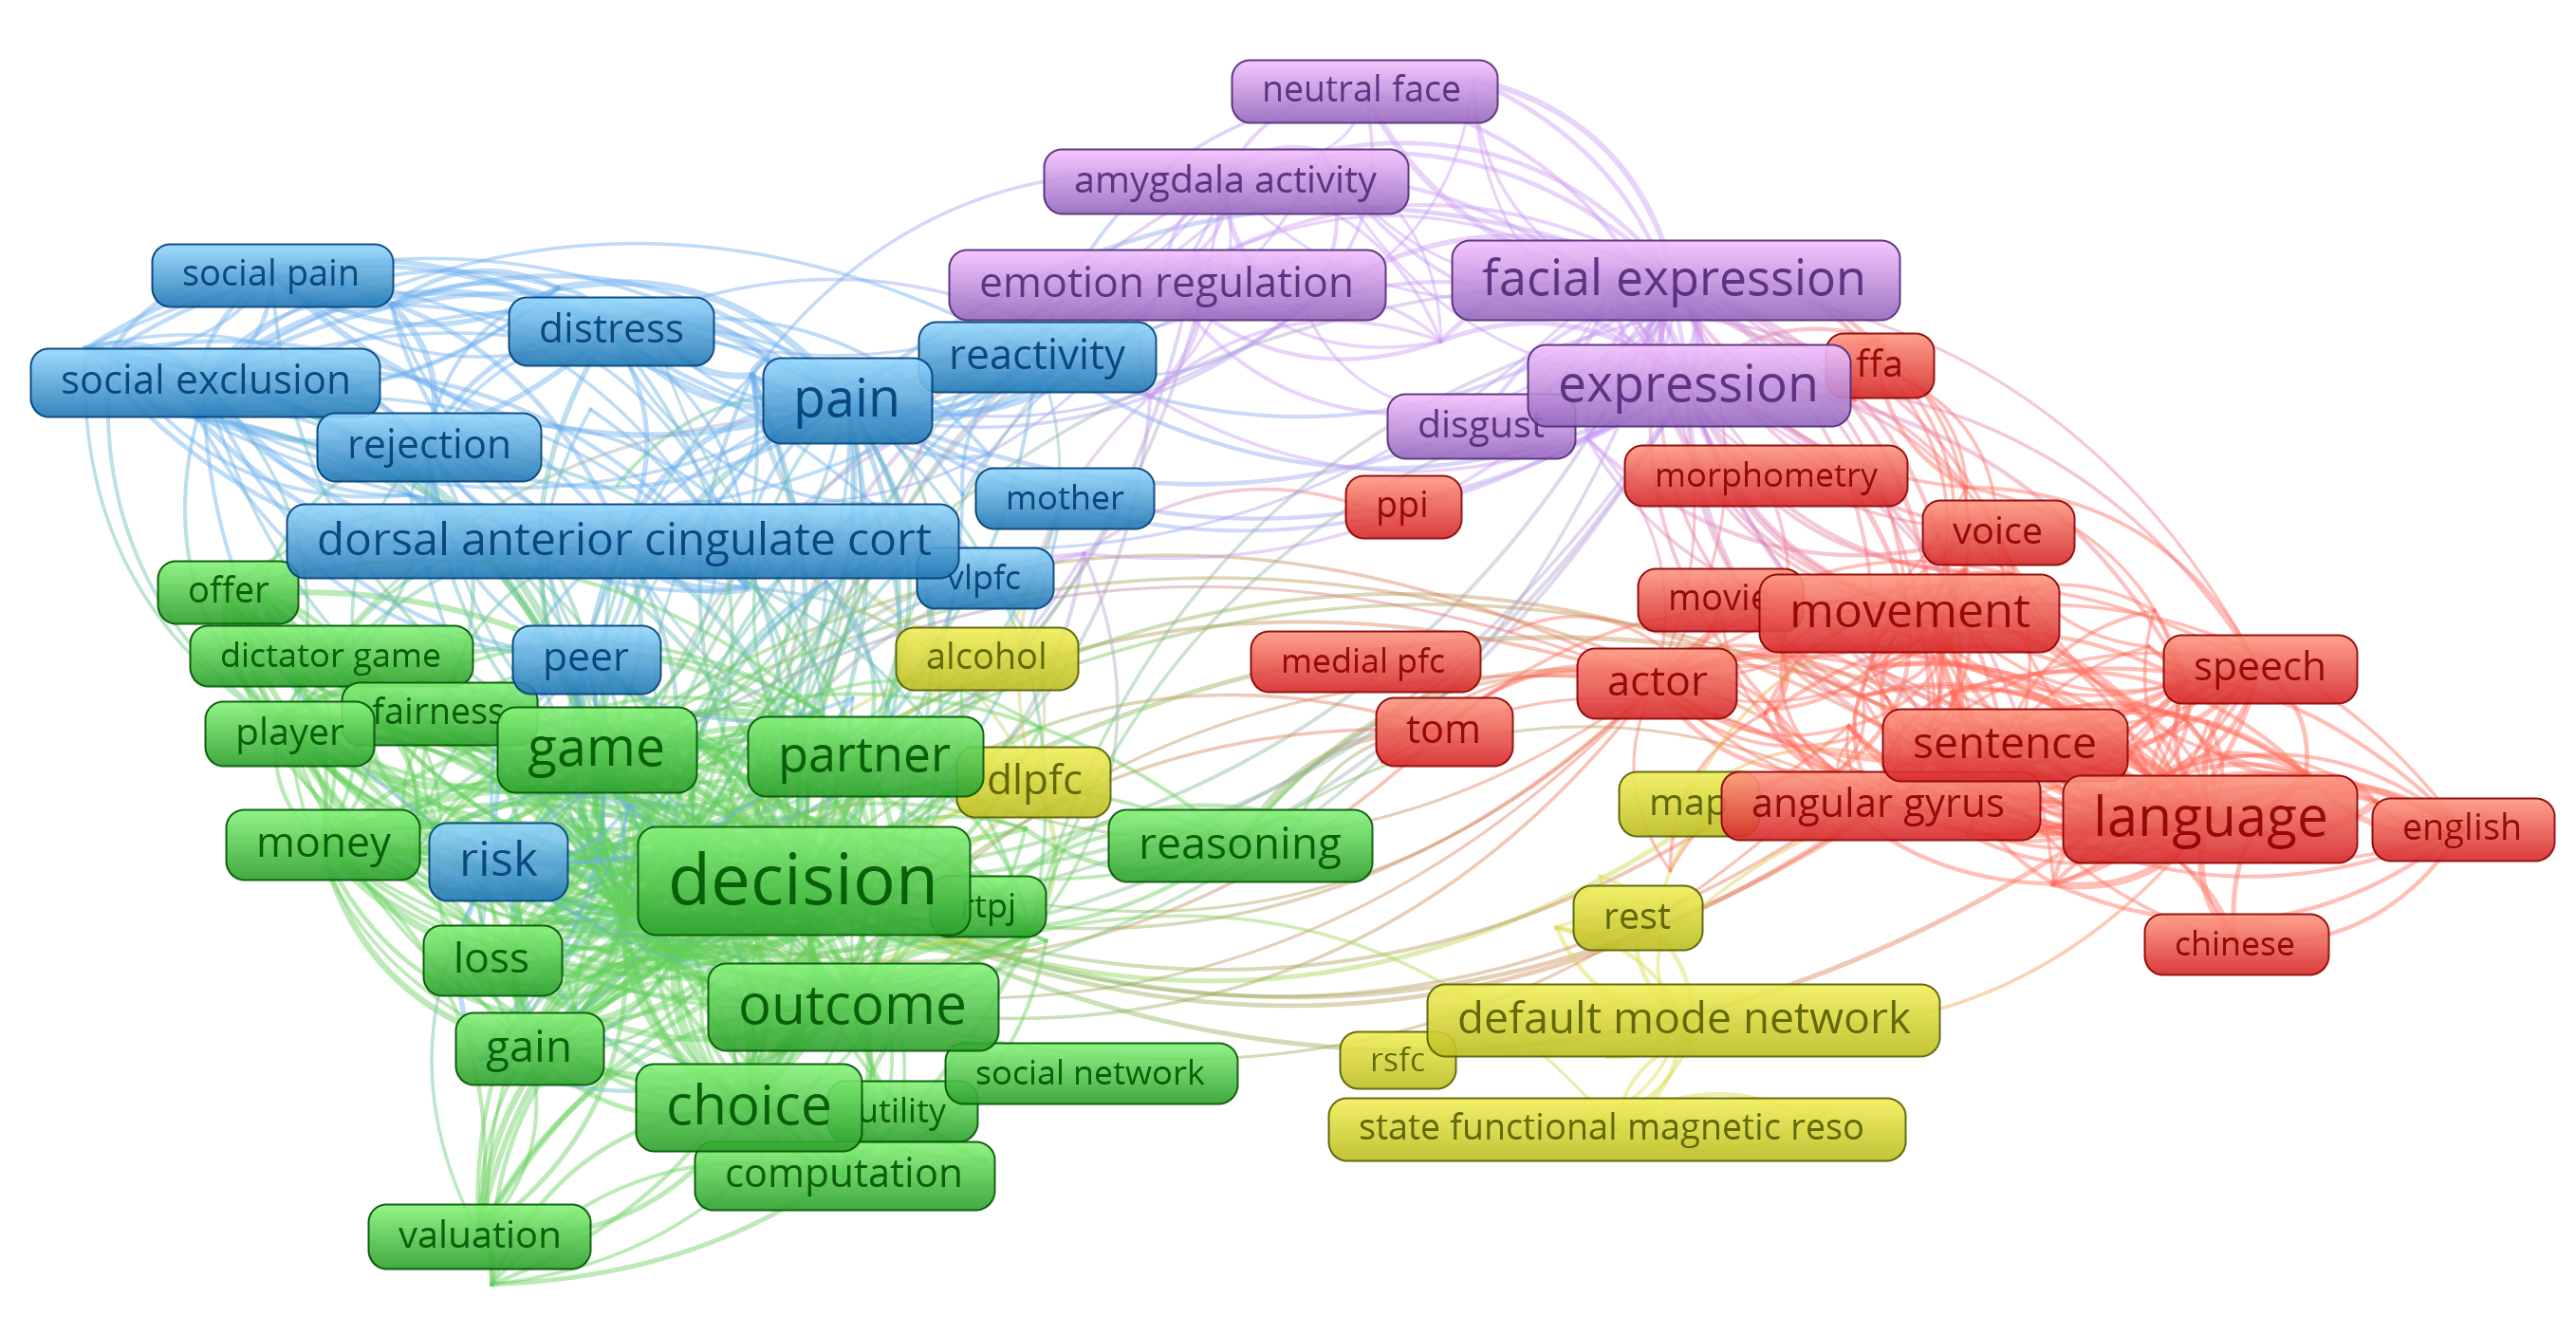
\includegraphics{vosviewer_label_cooccurence.png}
\caption{\textbf{Figure 3.} VOSviewer co-occurrence map of substantive keywords retrieved from the title and abstract of articles in our dataset. Colors represent VOSviewer-defined clusters of closely related keywords. See van Eck and Waltman (2014) for further details on clustering in VOSviewer. Online interactive version of the figure: \url{https://bit.ly/3yDPMup}}
\end{figure}

The VOSviewer co-occurrence map corroborates that themes commonly studied in social neuroscience frequently co-occur in the titles and abstracts of articles in our data. Further, the analysis shows that individual topics could be organized into larger categories based on keyword co-occurrence clusters {[}represented as keyword colors in Figure 3; van Eck and Waltman (2014){]}. As expected from a set of articles sampled from social neuroscience, these categories center around themes such as face perception (purple cluster), judgment and decision-making (green cluster), language (red cluster), and social pain/ostracism/exclusion (blue cluster). The default mode network (yellow cluster) also has clear ties to social neuroscience research (Li, Mai, \& Liu, 2014).

Converging lines of evidence suggest that our search strategy and selection process was successful in curating a dataset both representative of, and exclusive to our target population of healthy human social fMRI research. Note that our sampling and selection process was largely constructed to overcome the problem that social fMRI is not a well-defined bibliometric category. Determining an initial set of candidates will likely be more straightforward when the field of interest aligns more closely with a well-defined bibliometric category (e.g., a WoS field category).

We subsequently set out to quantitatively estimate the replication value for each study in this set (see Figure 1, step 2). Following Isager et al. (2021) we chose \emph{RV\textsubscript{Cn}} as our operationalization of replication value (equation 1). To quantify the replication value, researchers need to specify what function \(w\) should be used to weigh the citations, which type of citation impact \(C\) is used, as well as source \(S\) of that citation impact, if multiple sources are available. In the sections below we explain how citation impact and sample size data were collected in practice, and we explore the reliability of the collected data.

\hypertarget{operationalizing-value-as-citation-impact}{%
\subsubsection{Operationalizing value as citation impact}\label{operationalizing-value-as-citation-impact}}

To explore the impact of choosing one specification over another, we studied the reliability of citation impact estimates across a range of impact types \(C\), sources \(S\), and functions \(w\). Although changes to these values will immediately impact the absolute replication value that is calculated, we are mainly interested in their impact on the relative ranking of studies in terms of replication value. Two qualitatively different types of citation impact C were collected; traditional academic citation indexes and Altmetric attention scores. Altmetric attention scores were collected using the \emph{rAltmetric} package in R {[}Ram (2017); download date: 2020-10-30{]}. Altmetric attention scores are a weighted count of news- and social-media attention an article has received. For traditional citation impact, we collected data from multiple sources, including WoS (collected 2020-11-07 using the WoS web interface), Crossref (collected 2020-10-30 using the rCrossref package in R; Chamberlain, Zhu, Jahn, Boettiger, and Ram (2020)), Scopus (collected 2020-10-30 using the rScopus package in R; Muschelli (2019)), CWTS (collected 2020-10-28 from the CWTS database by author TvL), and scite™ (www.scite.ai; obtained 2021-08-23 by scite™ staff on request). WoS, Crossref, Scopus and scite™ citation counts are all unweighted raw counts of incoming citations of an article. CWTS citation counts consist only of incoming citations that are not self-citations. We also collected field- and age-normalized citation counts from the CWTS database. This normalization process corrects for differences between subfields in how often papers are cited on average, with the aim to treat publications from different fields equally (for details about the normalization procedure, and a discussion of the use of arithmetic averages in skewed distributions, see Waltman, van Eck, van Leeuwen, Visser, \& van Raan, 2011). The score represents how many more times the article is cited relative to the average citation count of an article in its field from the same year. Thus, our data contained three different functions \(w\) of traditional citation impact (raw count, self-citations subtracted, and field/age-normalized). Publication year data \(Y\) was collected from the WoS database.

\hypertarget{operationalizing-uncertainty-as-sample-size}{%
\subsubsection{Operationalizing uncertainty as sample size}\label{operationalizing-uncertainty-as-sample-size}}

Following the rationale of Isager et al. (2021) we operationalized the uncertainty about a claim before replication in terms of the standard error of effects supporting the claim. The standard error can be computed based on the standard deviation and the sample size, which is a combination of the number of participants and the number of observations per participant. We originally aimed to collect multiple sources of information that are relevant to quantifying the uncertainty such as information about the statistical test and the test results (e.g., the standard deviation of the dependent variable), the experimental design (e.g., the number of trials), the number of existing replications, etc., as such information can be used to compute and evaluate alternative operationalizations of replication value. This information would allow us to compare estimates from the \emph{RV\textsubscript{Cn}} indicator with other proposed indicators of replication value (e.g., Field et al., 2019, which requires information about bayes factors). We performed two pilot studies to 1) identify additional information that could be coded to quantify uncertainty, and 2) examine if this information could be efficiently coded (see supplementary materials SM2 and SM3, respectively). From these pilot studies we concluded that it was possible to identify the main claim in a paper (which was often feasible based on the abstract), but that is was not feasible to identify the results of the statistical test that provided empirical support for the main claim. It was often not possible to identify which of many statistical tests authors reported was the basis of the main claim, and therefore we were unable to extract the relevant statistical information to compute the replication value. Furthermore, statistical results were often not reported in sufficient detail to extract information (e.g., about the standard deviation of the measure). We concluded that it would not be feasible to collect additional information related to the uncertainty of the claim on a large scale from the social fMRI literature. In the end, the number of participants was the only operationalization of uncertainty we were able to move forward with in this study. This is an approximation of uncertainty that ignored variation in standard deviations, and the number of trials in a study, which is a topic we will return to in the general discussion.

\hypertarget{collecting-and-inspecting-the-reliability-of-rvcn-input}{%
\subsubsection{\texorpdfstring{Collecting and inspecting the reliability of \emph{RV\textsubscript{Cn}} input}{Collecting and inspecting the reliability of RVCn input}}\label{collecting-and-inspecting-the-reliability-of-rvcn-input}}

\hypertarget{reliability-of-citation-impact-across-sources}{%
\paragraph{Reliability of citation impact across sources}\label{reliability-of-citation-impact-across-sources}}

To better understand the relationship between different variables related to the citation impact \(C\) across sources \(S\), we explored the strength of the association between a variety of citation metrics (Table 3).

All metrics were retrieved within a time span of two weeks to prevent differences due to a time-lag. Figure 4 displays the distributions of all citation metrics. All metrics are heavily right skewed. The distributions of raw citation counts are highly overlapping across sources (Figure 4A). CWTS citation counts are more heavily skewed towards zero than raw counts from other metrics, likely due to the fact that CWTS subtracts self-citations from the total citation count.

\hfill\break

\begin{longtable}[]{@{}
  >{\centering\arraybackslash}p{(\columnwidth - 4\tabcolsep) * \real{0.2500}}
  >{\centering\arraybackslash}p{(\columnwidth - 4\tabcolsep) * \real{0.4583}}
  >{\centering\arraybackslash}p{(\columnwidth - 4\tabcolsep) * \real{0.0972}}@{}}
\caption{\textbf{Table 3:} Frequency of various citation metrics available for our data. Web of Science citation counts were originally available for all articles, but some could not be retrieved when the citation count data was updated in 2020.}\tabularnewline
\toprule()
\begin{minipage}[b]{\linewidth}\centering
citation.metric
\end{minipage} & \begin{minipage}[b]{\linewidth}\centering
description
\end{minipage} & \begin{minipage}[b]{\linewidth}\centering
N
\end{minipage} \\
\midrule()
\endfirsthead
\toprule()
\begin{minipage}[b]{\linewidth}\centering
citation.metric
\end{minipage} & \begin{minipage}[b]{\linewidth}\centering
description
\end{minipage} & \begin{minipage}[b]{\linewidth}\centering
N
\end{minipage} \\
\midrule()
\endhead
WoS & Web of Science Core Collection
Times Cited Count & 2105 \\
Crossref & Crossref citation counts & 2253 \\
Scopus & Scopus citation counts & 2238 \\
CWTS & CWTS citation counts -
excluding self-citations & 2220 \\
CWTS normalized & Total Field-Normalized
Citation Score. CWTS citation
impact of article relative to
the primary field to which the
article belongs. & 2220 \\
scite & The total scite citation count
from publication until year
2020. & 2091 \\
Altmetric & Altmetric score & 1874 \\
Total & Number of articles for which
all citation metrics were
available & 1590 \\
\bottomrule()
\end{longtable}

~

\begin{figure}
\centering
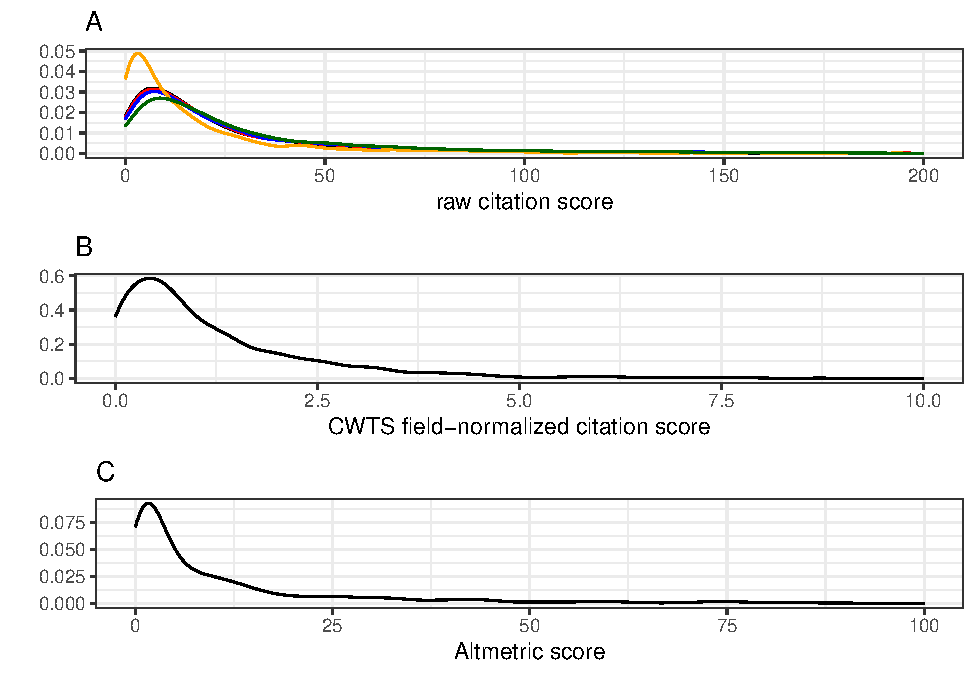
\includegraphics{RVcn_feasibility_in_social_neuroscience_cortex_files/figure-latex/fig4-1.pdf}
\caption{\label{fig:fig4}\textbf{Figure 4.} Density distribution of citation metrics up to 200 citations. \textbf{A)} The distribution of raw citation counts from Web of Science (black), Crossref (red), Scopus (blue) and CWTS (orange). \textbf{B)} The distribution of CWTS citation impact up to a score of 10, normalized by research field/cluster. \textbf{C)} The distribution of Altmetric attention scores up to 100.}
\end{figure}

To examine how strongly WoS, Crossref, Scopus, CWTS, and scite™ were correlated measures of the same underlying construct - the raw academic citation impact of an article - we subjected the citation data from these sources to an intraclass correlation analysis (model = two-way fixed effects, type = single rater, definition = consistency; Koo and Li (2016)) using the ICC function in the R package \emph{psych} (Revelle (2021); ICC3 output reported). Because all citation metrics have a skewed distribution, and because we are primarily concerned with the rank-ordering of studies we retrieved citation metrics for (\textbf{Isager2020?}) Spearman's rho correlation was used to assess the strength of association.

Figure 5 displays the rank-order correlations between various citation metrics. The correlation between raw citation counts from any two sources was very high (always \textgreater0.94). The inter-rater reliability between these metrics was similarly high, ICC = 0.97, CI95\%{[}0.96, 0.97{]}. When self-citations are subtracted, as is done in the CWTS citation counts, correlations are only ever so slightly slightly lower compared to intercorrelations between the other sources, suggesting that self-citations will not have a large impact the computation of a replication value.

\begin{figure}
\centering
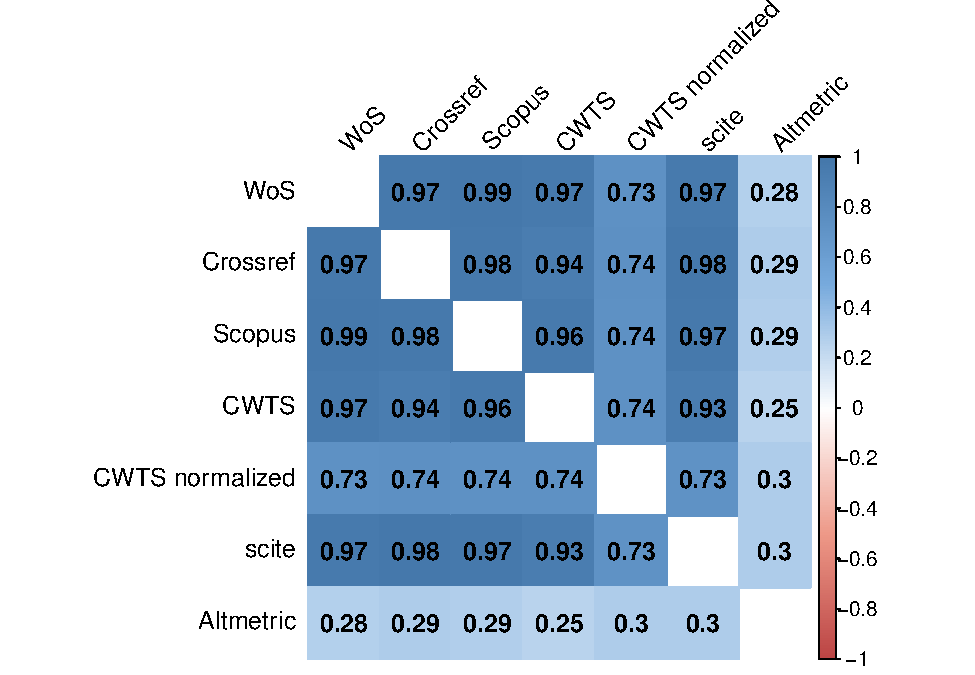
\includegraphics{RVcn_feasibility_in_social_neuroscience_cortex_files/figure-latex/fig5-1.pdf}
\caption{\label{fig:fig5}\textbf{Figure 5.} Matrix of bi-variate correlations between the citation metrics available for the articles in our dataset.}
\end{figure}

As expected based on the prior literature (Costas, Zahedi, \& Wouters, 2015) the correlations between Altmetric scores and all other metrics were consistently low. The correlation between normalized and non-normalized citation counts was consistently high across sources, though substantially lower than the inter-correlation between different raw citation counts. As will be discussed in more detail below, this suggests that it matters little for \emph{RV\textsubscript{Cn}} estimates which source \(S\) is used, but it does matter whether one chooses raw or field-normalized citation count as the operationalization of \(w(C)\), and it would matter substantially whether one chooses to use traditional citation count or news/social-media impact as the operationalization of \(C\). The reliability of Altmetric attention scores as estimates of news/social-media impact remains unclear, as we had no other metrics for this kind of impact to compare against. We will examine the consequences of using Altmetric scores or field-normalized citation counts on the computation of replication value scores below.

\hypertarget{accuracy-and-unbiasedness-of-average-yearly-citation-count.}{%
\paragraph{Accuracy and unbiasedness of average yearly citation count.}\label{accuracy-and-unbiasedness-of-average-yearly-citation-count.}}

The ideal citation metric of \emph{RV\textsubscript{Cn}} is the number of \emph{future} citations an article will receive (Isager et al., 2021). Total citation count would not be a useful estimator of future citation impact because citations accumulate over time. As an article gets older it will tend to get a higher total citation count regardless of expected future citations, which means that a 50 year old article cited once per year would have the total citations as an article published last year that has been cited 50 times, even though we should expect the latter to have much more impact on the field in the future. To prevent age from impacting the replication value of articles, \emph{RV\textsubscript{Cn}} uses the average yearly citation count instead of the total count as an operational measure of value.

To examine how well average yearly citation count predicts future citation count we obtained the yearly citation rate for each year separately from scite™, including the citation counts for 2020. Then, using the average yearly citation count of each article from using all years until 2019, we predicted the citation rate of each article in our data for year 2020 (the last complete year in the data from scite™). To examine whether average yearly citation count is a sufficient approach to correct for the effect of age on citation counts we examined the correlation between age and average yearly citation count. In addition, we explored the relationship between age-averaged citation count and age/field-normalized CWTS citation count, which are age-adjusted using the superior method of normalizing the citation count against all articles from the same year. If age-averaging is an effective method for age adjustment, age-averaged citation count should correlate more strongly with CWTS normalized scores than raw citation count. Finally, we also examined the effect of age-averaging on Altmetric attention scores. Our goal in examining the relationship between these variables is to gain a better understanding of which data should be used to quantify the value of a published study.

We focus on scite™ citation count data in these analyses since it was the only source from which we could obtain data on yearly citation rate. However, the reported pattern of results is highly similar regardless of which citation source is used (see supplementary material SM4).

\hypertarget{predictive-accuracy}{%
\subparagraph{Predictive accuracy}\label{predictive-accuracy}}

Figure 6A displays the scite™ citation rate trajectory for all articles in our data. Figure 6B displays the same trajectories on a log+1 scale with box plots summarizing the distribution for each year since publication, which gives a better sense of the overall trend. On average, most articles seem to be cited at an increasing rate for about the first two years since publication. Then the citation rate stabilizes, possibly increasing slightly around year ten. Given this general trend, our auxiliary assumption that average yearly citation count is on average a useful predictor of future citation impact is supported. Including citations from the two first years seems to leads to an underestimation of the citation rate in later years, but this might not directly affect any rank-order of citation counts.

\begin{figure}
\centering
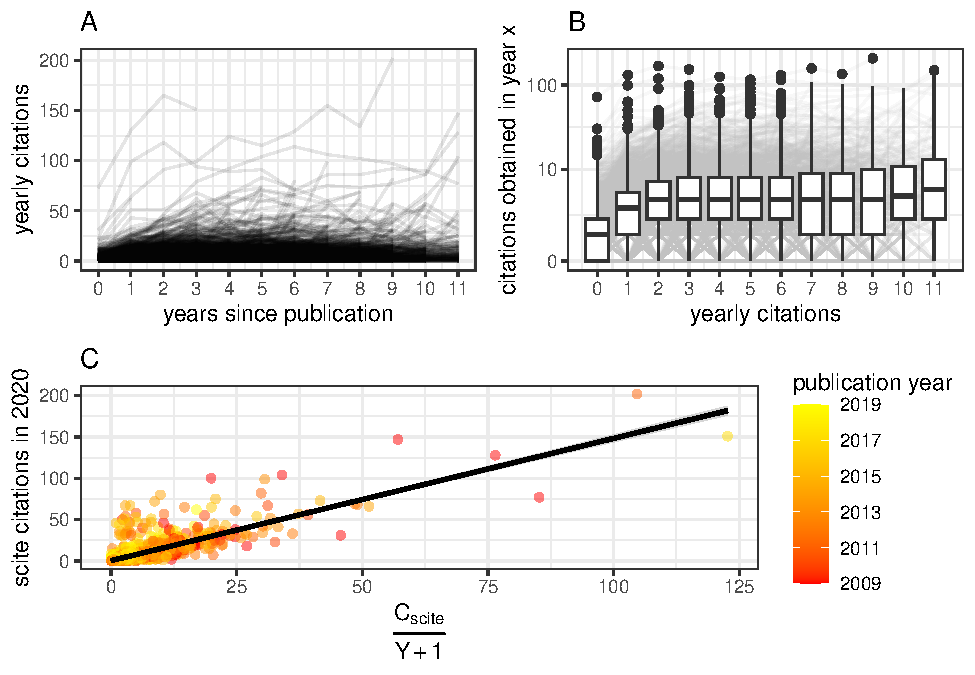
\includegraphics{RVcn_feasibility_in_social_neuroscience_cortex_files/figure-latex/fig6-1.pdf}
\caption{\label{fig:fig6}\textbf{Figure 6.} \textbf{A)} Citation trajectories for all articles in the dataset. \textbf{B)} Log citation trajectories, with box plot summaries for each year. \textbf{C)} Citations obtained in 2020 predicted by the average yearly citation count from the articles publication year until 2019.}
\end{figure}

Figure 6C displays the accuracy of average yearly citation count (using data until 2019) to predict the ``future'' citation count in 2020. Predictive accuracy is quite good, but far from perfect, \(\rho\) = 0.75, CI95\%{[}0.72, 0.77{]}. As noted above, average yearly citation count consistently underestimates how many citations are obtained in 2020. The two first years since publication are included in the average yearly citation count, which tends to drag down the average. Also as expected, underestimation of citations in 2020 seem to be particularly severe for more recently published articles. The younger the article, the more its average yearly citation count is influenced by the relatively lower number of yearly citations in the two first years since publication. Because total citation counts obtained from scite™ were highly correlated with total citation count obtained from other sources, we believe the results reported here likely generalizes to citations from WoS, Crossref, Scopus, and CWTS. The results suggest that the predictive accuracy of \emph{RV\textsubscript{Cn}} could be improved by excluding citations from the first two years since publication. Alternatively, accuracy could be improved through more accurate modeling of each article's citation trend. Such improvements require data on citations per year, which is not easily accessible to most researchers (the information was provided to us by scite™ (www.scite.ai)).

\hypertarget{predictive-unbiasedness}{%
\subparagraph{Predictive unbiasedness}\label{predictive-unbiasedness}}

Article age was very weakly correlated with the number of scite™ citations an article received from january to december of the year 2020, \(\rho\) = 0.07, CI95\%{[}0.02, 0.11{]}, suggesting article age is not a determinant of future citation impact and can safely be corrected for. To examine how well age-averaging corrects citation estimates for age, we computed pairwise spearman correlations between publication age, scite™ citation count, Altmetric scores, scite™ citation count divided by years since publication, Altmetric scores divided by years since publication, and CWTS normalized citation count.

\begin{figure}
\centering
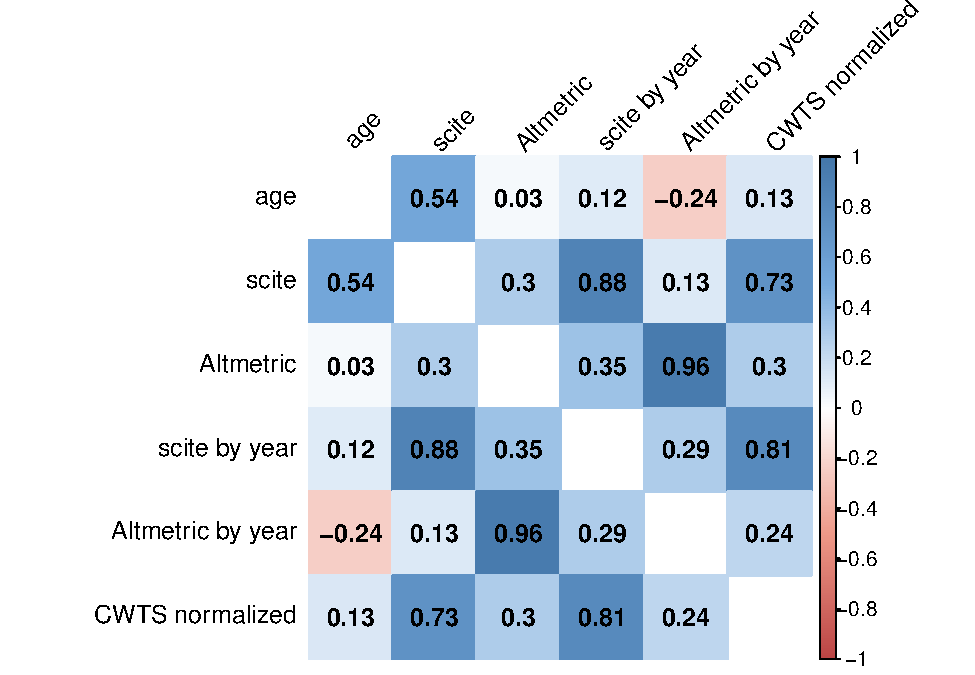
\includegraphics{RVcn_feasibility_in_social_neuroscience_cortex_files/figure-latex/fig7-1.pdf}
\caption{\label{fig:fig7}\textbf{Figure 7.} Matrix of bi-variate correlations between age and citation indices.}
\end{figure}

Figure 7 displays the correlation coefficients between all variables of interest. Not surprisingly, there was a strong correlation between age and raw scite™ citation count, \(\rho\) = 0.54, CI95\%{[}0.51, 0.57{]}. The correlation between citations and age dropped substantially when citation count was divided by years since publication. However, a small residual correlation between average yearly citation rate and publication age remains, \(\rho\) = 0.12, CI95\%{[}0.07, 0.16{]}. This suggests that dividing total citation count by the number of years since publication is an imperfect age adjustment method, but the correction substantially reduces the correlation between age and citation count, and is therefore a substantially better measure than total citation counts. Averaging over age works best if citation time accumulates at a constant rate, but this rate quite variable for most articles (Figure 6A). Encouragingly, however, averaging citation count by age does increase the correlation between citation count and CWTS normalized scores, whose method of age correction is superior as it corrects for the the average number of citations of all publications published in the same field and in the same year. Interestingly, even CWTS scores are weakly positively correlated with age, suggesting that perfectly adjusting for article age is challenging. In summary, taking the average yearly citation count seems to be an imperfect but efficient method for age adjustment in traditional citation metrics.

\hypertarget{coding-number-of-participants}{%
\paragraph{Coding number of participants}\label{coding-number-of-participants}}

The number of participants for each study in our dataset was coded manually. Manually coding the number of participants for all studies in the full set of 2268 candidate articles was assumed to be costly and time consuming from the outset. In practice, we expect most researchers to have more narrow inclusion criteria when computing the replication value for a set of replication targets. For feasibility reasons, we aimed at coding 1000 articles at random from the full set of 2268 articles and began the process of splitting these into individual studies for coding the number of participants. While coding, it became clear that many studies did not meet our inclusion criteria, and additional sample of 500 articles were sampled at random from the full set. The exact code used to draw the sample is available on OSF (\url{https://osf.io/rxukq/}). After removing articles that matched our initial exclusion criteria (e.g., single non-fMRI studies from multi-study articles, such as De Vries, Fennis, Bijmolt, Ter Horst, \& Marsman, 2018, study 4) the number of participants was coded for each fMRI study in the article.

Coding was performed by a team of three undergraduate research assistants. For each article we identified the number of studies reported in the article. For each study we recorded the number of participants who contributed any fMRI data to analyses reported in the study (even if their data were excluded from some analyses). For further details about how coders were instructed to proceed with coding the number of participants, see the supplementary coding instructions (\url{https://osf.io/j3pxf/}).

The 1500 articles contained 1681 individual studies, of which 323 matched our exclusion criteria. The final dataset contained 1358 individual studies from 1283 unique articles. Coding time was a few minutes when the number of participants and exclusion criteria were clearly summarized in either the study abstract or the ``participants'' subsection of the methods section, but could take longer if reporting was less structured. In order to ensure that the number of participants was reliably coded, a subset of 250 studies, randomly selected from the larger set of 1358, were double-coded by independent coders and subjected to an inter-rater reliability analysis. Two additional coders (one additional undergraduate student, the undergraduate coder, and the first author, the PhD coder) re-coded the number of participants for each study in this subset. While coding, all coders were blind to the number of participants provided by other coders. To study inter-rater reliability, we subsequently calculated the percentage agreement between each of the coders, and we calculated the intraclass correlation coefficient between coders (model = one-way fixed effects, type = single rater, definition = absolute agreement) using ICC function in the R package \emph{psych} (ICC3 output reported). Overall, there was a high but imperfect agreement between the three coders (percentage exact agreement = 0.77). The intraclass correlation coefficient between raters was high, ICC = 0.82, CI95\%{[}0.79, 0.86{]}. Figure 8 displays the variation in sample size between the coders, plotted on log scale.

\begin{figure}
\centering
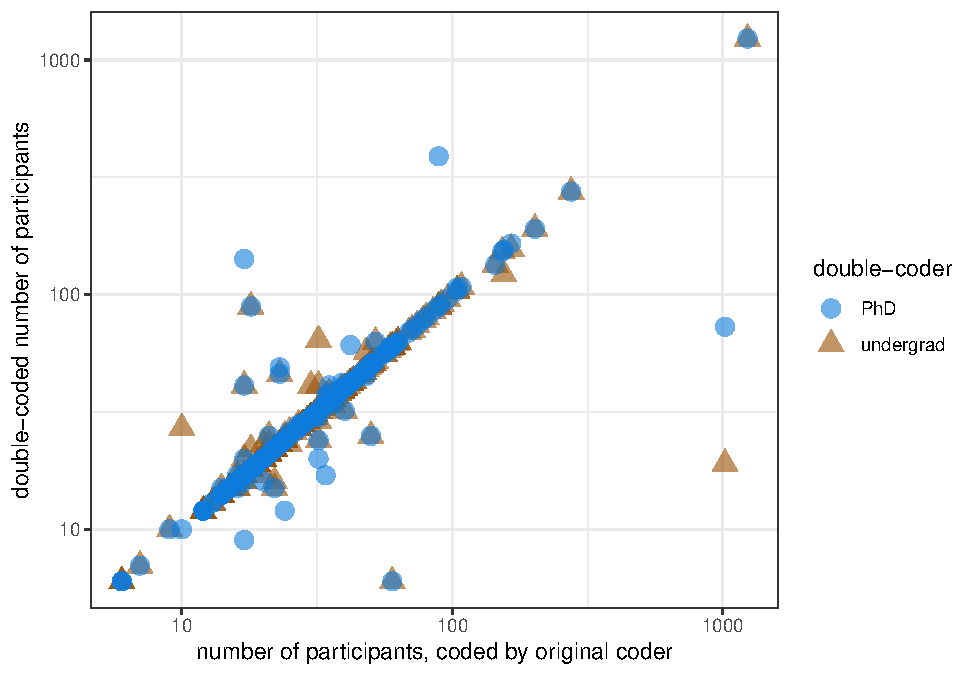
\includegraphics{RVcn_feasibility_in_social_neuroscience_cortex_files/figure-latex/fig8-1.pdf}
\caption{\label{fig:fig8}\textbf{Figure 8.} Variation in sample size between coders. Sample size is plotted on log scale. The original sample size coded is represented on the x-axis. Double-coded sample size values are represented on the y-axis. Blue circles represent values from the PhD-student coder. Brown triangles represent values from the undergraduate student coder.}
\end{figure}

Coders disagreed in 57 cases. All disagreements between coders were resolved by the PhD coder after inspecting comments by the other coders. In addition to the cases of disagreements identified in the data used for inter-rater reliability analysis, one additional sample size coding error in the full set of 1358 studies was detected and corrected at a later time during the analyses. Figure 9 displays the distribution of sample size in our data after resolving coder disagreements (mode=20, median=24, frequency of \emph{n\textless=10}=37, \emph{11-20}=479, \emph{21-30}=365, \emph{31-40}=184, \emph{41-50}=97, \emph{51-60}=60, \emph{61-70}=27, \emph{71-80}=25, \emph{81-90}=10, \emph{91-100}=10, \emph{n\textgreater100}=64).

\begin{figure}
\centering
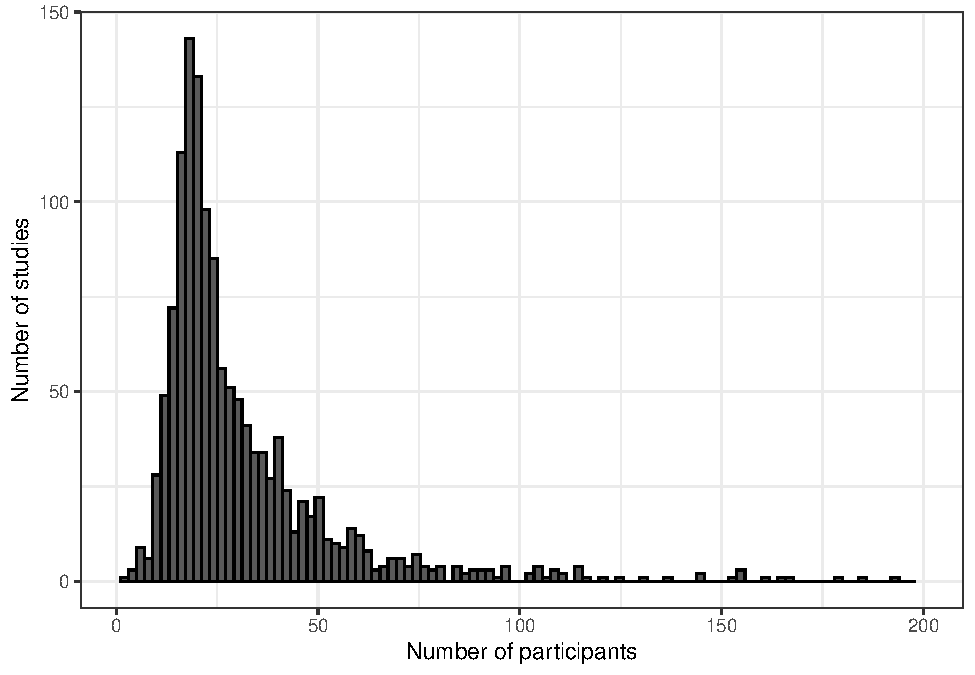
\includegraphics{RVcn_feasibility_in_social_neuroscience_cortex_files/figure-latex/fig9-1.pdf}
\caption{\label{fig:fig9}\textbf{Figure 9.} Distribution of sample sizes in the dataset. For visualization purposes, the x-axis limit is set to n = 200.}
\end{figure}

\hypertarget{calculating-and-comparing-alternative-operationalizations-of-rvcn}{%
\subsubsection{\texorpdfstring{Calculating and comparing alternative operationalizations of \emph{RV\textsubscript{Cn}}}{Calculating and comparing alternative operationalizations of RVCn}}\label{calculating-and-comparing-alternative-operationalizations-of-rvcn}}

Having established that sufficiently accurate citation counts and the number of participants can be collected, we proceeded with the calculation of \emph{RV\textsubscript{Cn}}. Because traditional citation counts are not strongly associated with Altmetric attention scores, replicating researchers might justifiably want to use either or both of these metrics to estimate value. Therefore, we decided to compare the results of several alternative operationalizations of replication value; one indicator measured value via the Web of Science citation count of the articles (\emph{RV\textsubscript{WoS}}), one via the Scopus citation count (\emph{RV\textsubscript{Scopus}}), one via the field-normalized citation counts (\emph{RV\textsubscript{tncs}}), one via the \emph{RV\textsubscript{scite}} and one indicator measured value via Altmetric score of the articles (\emph{RV\textsubscript{Alt}}). All indicators used sample size as a measure of uncertainty.

\emph{RV\textsubscript{WoS}} was based on the equations derived by Isager et al. (2021), and calculated in the following way:

\begin{equation} 
  \tag{2}
  RV_{WoS} = \frac{C_{WoS}}{Y+1}\times\frac{1}{\sqrt{n}}
  \label{eq:2}
\end{equation}

where \(C_{WoS}\) denotes the Web of Science citation count of the article a study is reported in, \(Y\) denotes the article age in years, and \(n\) denotes the sample size of the study after exclusion. The two measures using Scopus, scite™, and field-normalized citation scores were computed in the same way.

\emph{RV\textsubscript{Alt}} was calculated in the following way:

\begin{equation} 
  \tag{3}
  RV_{WoS} = C_{Alt}\times\frac{1}{\sqrt{n}}
  \label{eq:3}
\end{equation}

where \(C_{Alt}\) denotes the Altmetric attention score of the article, and \(n\) denotes the sample size of the study after exclusion. Because the analyses above revealed that Altmetric attention scores are not strongly correlated with article age in our data, we did not average \(C_{Alt}\) over publication year in this replication value indicator. Many articles are not mentioned in any sources that are tracked by Altmetric, and therefore have a score of 0. In our dataset \(C_{Alt}\) could only be calculated for 1156 of 1358 studies.

Importantly, we calculated all replication values under the assumption that no study in our candidate set is a replication of another study in the set, implying that no studies should be combined in the estimate of n.~Because lack of replication research in fMRI research (Poldrack et al., 2017) implies that only very few articles in our dataset would be replications of one another, we found it acceptable to proceed with calculation under the assumption that there were no replications in the data. Where direct replication studies have been performed, it would have been more appropriate to combine the sample size from the original study and it's replications (Isager et al., 2021, supplementary material 1). However, there are no databases that store information about direct replication in social neuroscience. Whenever researchers compute the replication value for a more specific population, information about direct replications might be more readily available, or it can be manually coded.

The distribution of replication value from all indicators was visually inspected, and estimates from indicators were correlated to study their similarity. Spearman's rho was used since the rank-order correlation between different indicators is of primary interest. 95\% bootstrap confidence intervals were calculated for the correlation estimate using the spearman.ci function of the RVAideMemoire package in R (Hervé, 2021).

\begin{figure}
\centering
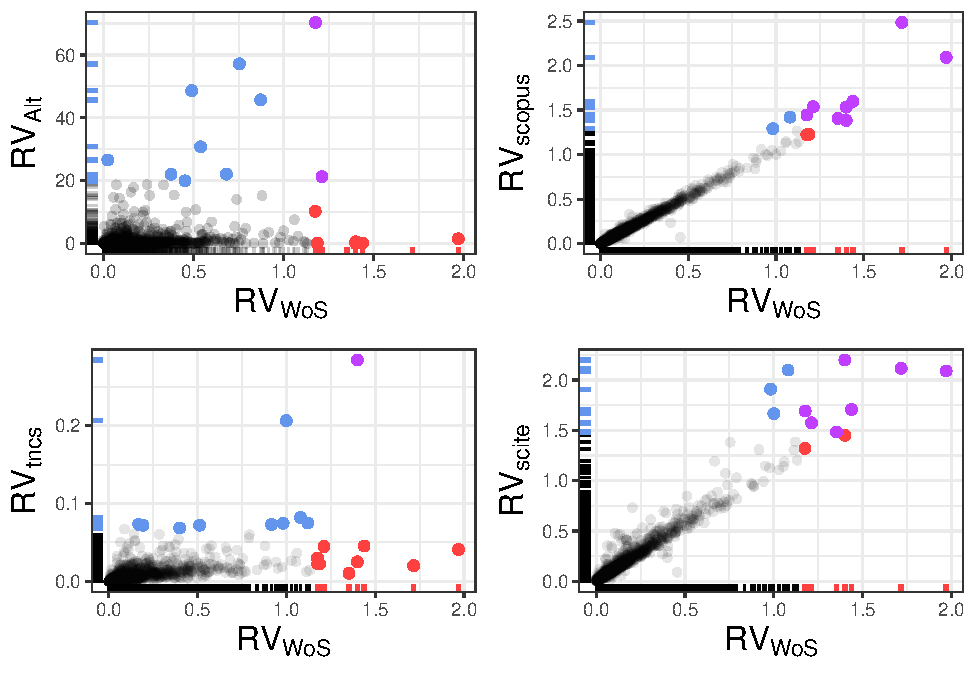
\includegraphics{RVcn_feasibility_in_social_neuroscience_cortex_files/figure-latex/fig10-1.pdf}
\caption{\label{fig:fig10}\textbf{Figure 10.} Scatter plot visualizing the relationship between \emph{RV\textsubscript{WoS}} and \emph{RV\textsubscript{Scopus}}, \emph{RV\textsubscript{tncs}}, \emph{RV\textsubscript{scite}}, and \emph{RV\textsubscript{Alt}}. Distribution of \emph{RV\textsubscript{WoS}} indicators are visualized as bars on the x-axis. Distribution of the other replication values are visualized as bars on the y-axis. Blue bars (and dots) represent the 10 highest scores on the y-axis. Red bars (and dots) represent the 10 highest \emph{RV\textsubscript{WoS}} scores. Purple dots represent scores that are among the 10 highest scores on both estimators. Two of the ten studies with the highest \emph{RV\textsubscript{WoS}} scores are not included in the scatter plot with the \emph{RV\textsubscript{Alt}} scores, as the \emph{RV\textsubscript{Alt}} could not be computed due to missing Altmetric attention scores.}
\end{figure}

Figure 10 displays the distribution of \emph{RV\textsubscript{WoS}}, \emph{RV\textsubscript{Alt}}, \emph{RV\textsubscript{Scopus}}, \emph{RV\textsubscript{tncs}} (field-normalized citation scores), \emph{RV\textsubscript{scite}}, and their associations with \emph{RV\textsubscript{WoS}}. Overall, all distributions are highly skewed with most scores distributed around low values, which is expected given that the number of participants, citation counts, and Altmetric attention scores are all highly skewed as well (see Figure 4 and Figure 9). Overall rank-order correlations were high for different citation sources (Web of Science, Scopus, scite), lower for field-normalized citation counts, and low for Altmetric scores (see Figure 11). As a consequence, only two studies (Kassam, Markey, Cherkassky, Loewenstein, \& Just, 2013; Tamir \& Mitchell, 2012) were ranked among the top ten in both Wob of Science and Altmetric rank-orderings (purple-colored points in Figure 10). The same was true for field-normalized citation scores, where the overlap between top-ranked studies using Web of Science citation scores and field-normalized citation scores was very low (despite the relatively high correlations between the two measures). Traditional citation impact and altmetric attention scores are generally thought to measure different aspects of impact and are known to be weakly associated. It is clear field-normalized citation scores also measure impact in a substantially different manner than raw citation counts. The overlap between citation counts from different sources such as scite™ or Scopus does not lead to substantially different selections, even though even there some variation in the last one or two studies included when selecting the X highest ranked studies (e.g., the 9th and 10th study included in a Top 10) should be expected to vary.

To conclude, quantitative recommendations for which studies to replicate will vary substantially based on whether traditional, field-normalized, or altmetric citation impact is used to estimate replication value, because these impact metrics measure non-overlapping aspects of scientific impact. Different stakeholders may prefer either operationalization, depending on what aspects of impact they find most relevant. Altmetric attention scores are only weakly correlated with traditional citation counts, which has a substantial impact on \emph{RV\textsubscript{Cn}} estimates.

\begin{figure}
\centering
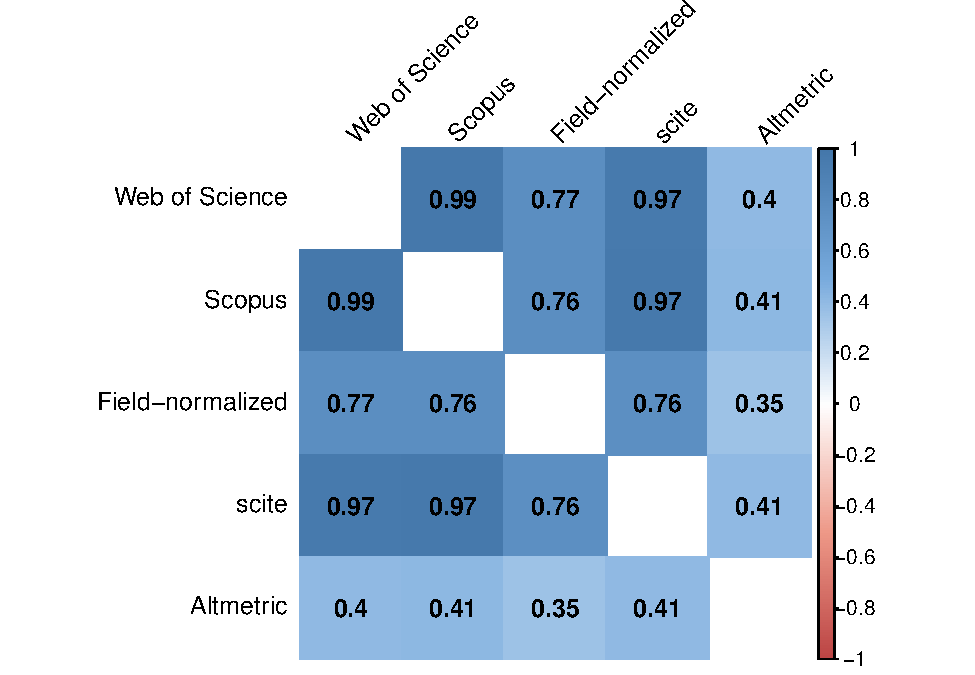
\includegraphics{RVcn_feasibility_in_social_neuroscience_cortex_files/figure-latex/fig11-1.pdf}
\caption{\label{fig:fig11}\textbf{Figure 11.} Matrix of bi-variate correlations between replication value indices computed based on different operationalizations of value through citations or Altmetrics.}
\end{figure}

\hypertarget{step-3---in-depth-review-of-recommended-candidates}{%
\subsection{Step 3 - In depth review of recommended candidates}\label{step-3---in-depth-review-of-recommended-candidates}}

The final step when selecting a replication target is an in-depth inspection of studies with a high replication value. We expect such an in-depth review to reveal certain boundary conditions of when the number of participants and/or the citation count do not accurately reflect the value and impact of a study. We subjected the 10 studies with the highest and lowest replication value on either \emph{RV\textsubscript{WoS}} or \emph{RV\textsubscript{Alt}} to an in-depth inspection. In addition, we included the 10 lowest non-zero estimates from the \emph{RV\textsubscript{WoS}} distribution, because \emph{RV\textsubscript{WoS}} scores of 0 often simply reflect a paper too young to have picked up citations yet. In total, 44 unique studies were included in our face validity review (6 studies were among the highest or lowest scores for both indicators).

We wanted to see whether quantitative replication value estimates would conform to our own intuitions about replication value, and identify factors that would lead to a high replication value using a formula-based approach, without actually warranting a replication. Such boundary conditions are likely present in other sets of replication targets as well, and identifying such factors will help researchers during the in-depth inspection in step 3. For example, an article may be highly cited for reasons other than the empirical studies it reportes, which would lead to a highly cited paper while the study in the article is not worth replicating. As such, the goal is to identify potential issues with validity, reliability and measurement error that future validation studies of \emph{RV\textsubscript{Cn}} may want to follow up on.

Authors PMI and AvtV read the title and abstracts of all studies included in the review, consulted the article text intermittently for clarifications, and reviewed quantitative information related to the replication value estimates of these studies (i.e., reviewers were not blinded to a record's rank position). Both reviewers first made notes for each study in private, focusing on their intuitive validity judgment of the replication value estimate and on potential sources of error and bias. Notes were then discussed by PMI, AvtV, and DL in two meetings to distill the most central outcomes of the review effort. The full set of notes is available on OSF for author PMI (\url{https://osf.io/vwpqs/}) and AvtV (\url{https://osf.io/953rh/}).

\hypertarget{central-outcomes-of-the-review-process}{%
\subsubsection{Central outcomes of the review process}\label{central-outcomes-of-the-review-process}}

The in-depth review yielded several insights. A detailed inspection of quantitative replication value estimates is important for quality control. In two studies, coders had erroneously coded an incorrect number of participants (due to a transcription error, and overlooking data exclusions). Eight articles turned out not to be connected to social neuroscience, and one study did not utilize fMRI for imaging. Finally, in one case we had incorrectly labeled a single two-session repeated measures study as two separate studies.

There was not always an intuitive correspondence between the \emph{RV\textsubscript{WoS}}/\emph{RV\textsubscript{Alt}} rank order and our intuitions about the replication value of the claims purely based on the title and information in the abstract. One reason for the lack for the correspondence was because reviewers were not blind to the replication value ranking, and had access to the citation count and number of participants, which were so salient they were difficult to not take into account. Another reason was that without other explicit criteria determining to determine the value of a replication study, there was substantial subjectivity in the value of each study as judged by both reviewers. This is not unexpected, as peer evaluations of the value of a study is variable, and not strongly related to eventual citation scores (Gottfredson, 1978). A final reason for the low perceived correspondence between indicator estimates and reviewer intuitions were a number of boundary conditions where the \emph{RV\textsubscript{WoS}}/\emph{RV\textsubscript{Alt}} estimates did not accurately reflect the value and uncertainty of the studies.

The first boundary condition was that many studies used within-subject designs, where the number of participants does not fully capture the uncertainty, as it ignores the number of measurements per participant. The use of within-subject designs seemed to be common among the highest ranked studies, as such designs require less participants for high statistical power, and therefore get a higher replication value when uncertainty is based only on the number of participants. This is clearly an important limitation, especially when the number of trials in each study varies substantially between studies (as was the case in the set of studies we examined). In future applications of \emph{RV\textsubscript{Cn}}-based study selection we therefore recommend that uncertainty is quantified during step 2 based on both the number of participants, and the number of observations per participant. If this is unfeasible (which is likely given how unsystematically this information is reported in the literature), the number of observations should be taken into account during step 3 (see supplementary material 2 in Isager et al., 2021 for technical details on such a correction method). Another boundary condition concerned a study that already had been replicated in the literature. Although rare, when replication studies already exist, the replication value should be computed based on the uncertainty remaining after all replication studies (\textbf{Isager2020?}).

Other boundary conditions concerned the reason an article is highly cited. One article containing both a literature review and an empirical study seemed to be cited primarily due to the literature review (Dimoka, Pavlou, \& Davis, 2011). Another study on human navigation appeared to receive a large Altmetric score primarily due to speculative news reports claiming that GPS use can ``turn the brain off'' - even though this conclusion did not follow from the study (Javadi et al., 2017). Researchers might want to reflect on whether the solution to a dubious interpretation of the results of a study warrant a replication study. The boundary conditions identified so far seem general enough to incorporate in the in-depth review process of replication targets by default. Future research should give us a better understanding of which additional factors to consider during in-depth review of replication candidates (e.g., Pittelkow et al., 2023).

\hypertarget{general-discussion}{%
\section{General discussion}\label{general-discussion}}

The overall aim of this exploratory study was to test the feasibility of implementing the four-step replication study selection procedure based on \emph{RV\textsubscript{Cn}} proposed by Isager et al. (2021) in social fMRI research. The current exploratory report reveals the importance of testing the feasibility of applying recently proposed selection strategies for replication studies, as well as carefully examining possible measures, auxiliary assumptions, and boundary conditions. We show it is possible to calculate \emph{RV\textsubscript{Cn}} for a large candidate set of studies identified based on bibliometric information. We were able to reliably code the total number of participants and retrieve citation count data for each study in order to calculate \emph{RV\textsubscript{Cn}} (step 2 in Figure 1). However, we were only able to code uncertainty coarsely as `number of participants in study', omitting the number of trials per participant, which also determines the standard error of the estimate (Westfall, Kenny, \& Judd, 2014).

Traditional citation count metrics were highly rank-order correlated, meaning there is little difference in which source \(S\) is used in the calculation of \emph{RV\textsubscript{Cn}}. Field-normalized citation counts provide a somewhat different measure of citation impact, and lead to less overlap in the final rank-order than non-normalized citation scores, especially in an interdisciplinary research topic such as social neuroscience, where publication appear across scientific fields, which leads to different articles being normalized against different field-wide averages. Altmetric attention scores are weakly correlated with traditional citation impact, and represent a qualitatively different approach to measuring value. Whichever measure is preferred, both Altmetric scores, traditional citation counts could easily be extracted using free and open source applications (Chamberlain et al., 2020; e.g., Ram, 2017), where field-normalized citation counts or citation counts per year are not publicly available.

Finally, in-depth review of the highest ranking indicator estimates from step 2 appears to be an important method of quality control before a candidate is selected for replication. This review revealed important boundary conditions of using citation counts and the total number of participants as measures of value and uncertainty. Auxiliary hypotheses, such that past citation counts predict future citation counts, that the source of the citation counts do not substantially affect the rank-order, and that we can control for the age of the article, were all supported.

Whether these conclusions generalize to application of \emph{RV\textsubscript{Cn}} in other disciplines is an open question which will need to be empirically examined. Our initial set of replication targets was large and heterogeneous, and the use of \emph{RV\textsubscript{Cn}} might be more straightforward in more homogenous literatures, especially if these mainly rely on between-participant designs. Ideally, we would validate any quantification of replication value by benchmarking the quantitative estimates against a reliable measure of expected utility gain. However, such benchmark validation will be highly difficult to implement in practice, as utility judgments are difficult to quantify, and would require extensive discussions among peers in a specific research area to reach consensus about which studies are most valuable to replicate.

One could attempt to provide criterion validation of \emph{RV\textsubscript{Cn}} by investigating whether \emph{RV\textsubscript{Cn}} is associated with other operational measures that are hypothesized to predict expected utility gain. For example, we would expect \emph{RV\textsubscript{Cn}} to predict which studies are chosen for replication in practice under the assumption that both \emph{RV\textsubscript{Cn}} and the selection criteria used by researchers who perform replication studies are caused by the expected utility of the replication effort (Isager et al., 2021).It might also be possible to validate \emph{RV\textsubscript{Cn}} by examining the extent to which \emph{RV\textsubscript{Cn}} predicts subjective estimates of the relative replication value of a set of studies. Future studies could also aim to increase the understanding of which factors researchers usually consider when selecting a study for replication. Recently, Pittelkow et al. (2023) identified a number of criteria such as interest, doubt, impact, methodology, and feasibility. An important next step is to examine how feasible it is to quantify these factors, and how well such judgments relate to \emph{RV\textsubscript{Cn}}. It is important that measures of \emph{RV\textsubscript{Cn}} should not be predictive of whether a study will replicate successfully. \emph{RV\textsubscript{Cn}} estimates should be the highest for studies we cannot accurately predict replication outcomes for, and therefore studies that are either very likely to replicate or very unlikely to replicate should \emph{both} receive low \emph{RV\textsubscript{Cn}}.

The task of evaluating the uncertainty in scientific claims would have been made easier if researchers adhered to reporting standards, and when the relationship between statistical tests and scientific claims were more clearly specified in the article (Appelbaum et al., 2018; Lakens \& DeBruine, 2021). Furthermore, it would be beneficial if researchers who perform replication studies are explicit about the reasons they selected a target study (Pittelkow et al., 2023). By exploring and documenting the wealth of information relevant to replication study selection, we can increase the ability of researchers to make well-informed decisions about which original research would be the most important to replicate.

\hypertarget{references}{%
\section*{References}\label{references}}
\addcontentsline{toc}{section}{References}

\hypertarget{refs}{}
\begin{CSLReferences}{1}{0}
\leavevmode\vadjust pre{\hypertarget{ref-appelbaum_journal_2018}{}}%
Appelbaum, M., Cooper, H., Kline, R. B., Mayo-Wilson, E., Nezu, A. M., \& Rao, S. M. (2018). Journal article reporting standards for quantitative research in psychology: {The APA Publications} and {Communications Board} task force report. \emph{American Psychologist}, \emph{73}(1), 3--25. \url{https://doi.org/10.1037/amp0000191}

\leavevmode\vadjust pre{\hypertarget{ref-Ashar2021}{}}%
Ashar, Y. K., Clark, J., Gunning, F. M., Goldin, P., Gross, J. J., \& Wager, T. D. (2021). Brain markers predicting response to cognitive-behavioral therapy for social anxiety disorder: An independent replication of {Whitfield}-{Gabrieli} et al. 2015. \emph{Translational Psychiatry}, \emph{11}(1), 260. \url{https://doi.org/10.1038/s41398-021-01366-y}

\leavevmode\vadjust pre{\hypertarget{ref-Boekel2015}{}}%
Boekel, W., Wagenmakers, E.-J., Belay, L., Verhagen, J., Brown, S., \& Forstmann, B. U. (2015). A purely confirmatory replication study of structural brain-behavior correlations. \emph{Cortex}, \emph{66}, 115--133. \url{https://doi.org/10.1016/j.cortex.2014.11.019}

\leavevmode\vadjust pre{\hypertarget{ref-Botvinik-Nezer2020}{}}%
Botvinik-Nezer, R., Holzmeister, F., Camerer, C. F., Dreber, A., Huber, J., Johannesson, M., \ldots{} Schonberg, T. (2020). Variability in the analysis of a single neuroimaging dataset by many teams. \emph{Nature}, \emph{582}(7810), 84--88. \url{https://doi.org/10.1038/s41586-020-2314-9}

\leavevmode\vadjust pre{\hypertarget{ref-Button2013}{}}%
Button, K. S., Ioannidis, J. P. A., Mokrysz, C., Nosek, B. A., Flint, J., Robinson, E. S. J., \& Munafò, M. R. (2013). Power failure: Why small sample size undermines the reliability of neuroscience. \emph{Nature Reviews Neuroscience}, \emph{14}(5), 365--376. \url{https://doi.org/10.1038/nrn3475}

\leavevmode\vadjust pre{\hypertarget{ref-Carp2012}{}}%
Carp, J. (2012). On the {Plurality} of ({Methodological}) {Worlds}: {Estimating} the {Analytic Flexibility} of {fMRI Experiments}. \emph{Frontiers in Neuroscience}, \emph{6}. \url{https://doi.org/10.3389/fnins.2012.00149}

\leavevmode\vadjust pre{\hypertarget{ref-Chamberlain2020}{}}%
Chamberlain, S., Zhu, H., Jahn, N., Boettiger, C., \& Ram, K. (2020). \emph{Rcrossref}.

\leavevmode\vadjust pre{\hypertarget{ref-Costas2015}{}}%
Costas, R., Zahedi, Z., \& Wouters, P. (2015). Do {``altmetrics''} correlate with citations? {Extensive} comparison of altmetric indicators with citations from a multidisciplinary perspective. \emph{Journal of the Association for Information Science and Technology}, \emph{66}(10), 2003--2019. \url{https://doi.org/10.1002/asi.23309}

\leavevmode\vadjust pre{\hypertarget{ref-DeVries2018}{}}%
De Vries, E. L. E., Fennis, B. M., Bijmolt, T. H. A., Ter Horst, G. J., \& Marsman, J.-B. C. (2018). Friends with benefits: {Behavioral} and {fMRI} studies on the effect of friendship reminders on self-control for compulsive and non-compulsive buyers. \emph{International Journal of Research in Marketing}, \emph{35}(2), 336--358. \url{https://doi.org/10.1016/j.ijresmar.2017.12.004}

\leavevmode\vadjust pre{\hypertarget{ref-Dimoka2011}{}}%
Dimoka, A., Pavlou, P. A., \& Davis, F. D. (2011). {NeuroIS}: {The Potential} of {Cognitive Neuroscience} for {Information Systems Research}. \emph{Information Systems Research}, \emph{22}(4), 687--702. \url{https://doi.org/10.1287/isre.1100.0284}

\leavevmode\vadjust pre{\hypertarget{ref-Federer2018}{}}%
Federer, L. M., Belter, C. W., Joubert, D. J., Livinski, A., Lu, Y.-L., Snyders, L. N., \& Thompson, H. (2018). Data sharing in {PLOS ONE}: {An} analysis of {Data Availability Statements}. \emph{PLOS ONE}, \emph{13}(5), e0194768. \url{https://doi.org/10.1371/journal.pone.0194768}

\leavevmode\vadjust pre{\hypertarget{ref-Field2019}{}}%
Field, S. M., Hoekstra, R., Bringmann, L., \& Van Ravenzwaaij, D. (2019). When and {Why} to {Replicate}: {As Easy} as 1, 2, 3? \emph{Collabra: Psychology}, \emph{5}(1), 46. \url{https://doi.org/10.1525/collabra.218}

\leavevmode\vadjust pre{\hypertarget{ref-Furukawa2006}{}}%
Furukawa, T. A., Barbui, C., Cipriani, A., Brambilla, P., \& Watanabe, N. (2006). Imputing missing standard deviations in meta-analyses can provide accurate results. \emph{Journal of Clinical Epidemiology}, \emph{59}(1), 7--10. \url{https://doi.org/10.1016/j.jclinepi.2005.06.006}

\leavevmode\vadjust pre{\hypertarget{ref-Glasziou2008}{}}%
Glasziou, P., Meats, E., Heneghan, C., \& Shepperd, S. (2008). What is missing from descriptions of treatment in trials and reviews? \emph{BMJ}, \emph{336}(7659), 1472--1474. \url{https://doi.org/10.1136/bmj.39590.732037.47}

\leavevmode\vadjust pre{\hypertarget{ref-gottfredson_evaluating_1978}{}}%
Gottfredson, S. D. (1978). Evaluating psychological research reports: {Dimensions}, reliability, and correlates of quality judgments. \emph{American Psychologist}, \emph{33}, 920--934. \url{https://doi.org/10.1037/0003-066X.33.10.920}

\leavevmode\vadjust pre{\hypertarget{ref-Heirene2021}{}}%
Heirene, R. M. (2021). A call for replications of addiction research: Which studies should we replicate and what constitutes a {``successful''} replication? \emph{Addiction Research \& Theory}, \emph{29}(2), 89--97. \url{https://doi.org/10.1080/16066359.2020.1751130}

\leavevmode\vadjust pre{\hypertarget{ref-Herve2021}{}}%
Hervé, M. (2021). \emph{{RVAideMemoire}: {Testing} and {Plotting Procedures} for {Biostatistics}}.

\leavevmode\vadjust pre{\hypertarget{ref-Huber2019}{}}%
Huber, D. E., Potter, K. W., \& Huszar, L. D. (2019). Less {``{Story}''} and more {``{Reliability}''} in cognitive neuroscience. \emph{Cortex; a Journal Devoted to the Study of the Nervous System and Behavior}, \emph{113}, 347--349. \url{https://doi.org/10.1016/j.cortex.2018.10.030}

\leavevmode\vadjust pre{\hypertarget{ref-Isager2021}{}}%
Isager, P. M., Veer, A. van 't, \& Lakens, D. (2021). \emph{Replication value as a function of citation impact and sample size}. {MetaArXiv}. \url{https://doi.org/10.31222/osf.io/knjea}

\leavevmode\vadjust pre{\hypertarget{ref-Javadi2017}{}}%
Javadi, A.-H., Emo, B., Howard, L. R., Zisch, F. E., Yu, Y., Knight, R., \ldots{} Spiers, H. J. (2017). Hippocampal and prefrontal processing of network topology to simulate the future. \emph{Nature Communications}, \emph{8}(1), 14652. \url{https://doi.org/10.1038/ncomms14652}

\leavevmode\vadjust pre{\hypertarget{ref-Kassam2013}{}}%
Kassam, K. S., Markey, A. R., Cherkassky, V. L., Loewenstein, G., \& Just, M. A. (2013). Identifying {Emotions} on the {Basis} of {Neural Activation}. \emph{PLoS ONE}, \emph{8}(6), e66032. \url{https://doi.org/10.1371/journal.pone.0066032}

\leavevmode\vadjust pre{\hypertarget{ref-KNAW2018}{}}%
KNAW. (2018). \emph{Replication studies \textendash{} {Improving} reproducibility in the empirical sciences}. {Amsterdam}: {KNAW}.

\leavevmode\vadjust pre{\hypertarget{ref-Koo2016}{}}%
Koo, T. K., \& Li, M. Y. (2016). A {Guideline} of {Selecting} and {Reporting Intraclass Correlation Coefficients} for {Reliability Research}. \emph{Journal of Chiropractic Medicine}, \emph{15}(2), 155--163. \url{https://doi.org/10.1016/j.jcm.2016.02.012}

\leavevmode\vadjust pre{\hypertarget{ref-lakens_improving_2021}{}}%
Lakens, D., \& DeBruine, L. M. (2021). Improving {Transparency}, {Falsifiability}, and {Rigor} by {Making Hypothesis Tests Machine-Readable}. \emph{Advances in Methods and Practices in Psychological Science}, \emph{4}(2), 2515245920970949. \url{https://doi.org/10.1177/2515245920970949}

\leavevmode\vadjust pre{\hypertarget{ref-Li2014}{}}%
Li, W., Mai, X., \& Liu, C. (2014). The default mode network and social understanding of others: What do brain connectivity studies tell us. \emph{Frontiers in Human Neuroscience}, \emph{0}. \url{https://doi.org/10.3389/fnhum.2014.00074}

\leavevmode\vadjust pre{\hypertarget{ref-Matiasz2018}{}}%
Matiasz, N. J., Wood, J., Doshi, P., Speier, W., Beckemeyer, B., Wang, W., \ldots{} Silva, A. J. (2018). {ResearchMaps}.org for integrating and planning research. \emph{PloS One}, \emph{13}(5), e0195271. \url{https://doi.org/10.1371/journal.pone.0195271}

\leavevmode\vadjust pre{\hypertarget{ref-Muschelli2019}{}}%
Muschelli, J. (2019). \emph{Rscopus: {Scopus Database} '{API}' {Interface}}.

\leavevmode\vadjust pre{\hypertarget{ref-pittelkow_process_2023}{}}%
Pittelkow, M.-M., Field, S. M., Isager, P. M., van't Veer, A. E., Anderson, T., Cole, S. N., \ldots{} van Ravenzwaaij, D. (2023). The process of replication target selection in psychology: What to consider? \emph{Royal Society Open Science}, \emph{10}(2), 210586. \url{https://doi.org/10.1098/rsos.210586}

\leavevmode\vadjust pre{\hypertarget{ref-Poldrack2017}{}}%
Poldrack, R. A., Baker, C. I., Durnez, J., Gorgolewski, K. J., Matthews, P. M., Munafò, M. R., \ldots{} Yarkoni, T. (2017). Scanning the horizon: Towards transparent and reproducible neuroimaging research. \emph{Nature Reviews Neuroscience}, \emph{18}(2), 115--126. \url{https://doi.org/10.1038/nrn.2016.167}

\leavevmode\vadjust pre{\hypertarget{ref-Ram2017}{}}%
Ram, K. (2017). \emph{{rAltmetric}: {Retrieves Altmerics Data} for {Any Published Paper} from '{Altmetric}.com'}.

\leavevmode\vadjust pre{\hypertarget{ref-Revelle2021}{}}%
Revelle, W. (2021). \emph{Psych: {Procedures} for {Psychological}, {Psychometric}, and {Personality Research}}.

\leavevmode\vadjust pre{\hypertarget{ref-scheel_why_2021}{}}%
Scheel, A. M., Tiokhin, L., Isager, P. M., \& Lakens, D. (2021). Why {Hypothesis Testers Should Spend Less Time Testing Hypotheses}. \emph{Perspectives on Psychological Science}, \emph{16}(4), 744--755. \url{https://doi.org/10.1177/1745691620966795}

\leavevmode\vadjust pre{\hypertarget{ref-schmidt_shall_2009}{}}%
Schmidt, S. (2009). Shall we really do it again? {The} powerful concept of replication is neglected in the social sciences. \emph{Review of General Psychology}, \emph{13}(2), 90--100. \url{https://doi.org/10.1037/a0015108}

\leavevmode\vadjust pre{\hypertarget{ref-Sullivan2012}{}}%
Sullivan, G. M., \& Feinn, R. (2012). Using {Effect Size}\textemdash or {Why} the {P Value Is Not Enough}. \emph{Journal of Graduate Medical Education}, \emph{4}(3), 279--282. \url{https://doi.org/10.4300/JGME-D-12-00156.1}

\leavevmode\vadjust pre{\hypertarget{ref-Szucs2017}{}}%
Szucs, D., \& Ioannidis, J. P. A. (2017). Empirical assessment of published effect sizes and power in the recent cognitive neuroscience and psychology literature. \emph{PLOS Biology}, \emph{15}(3), e2000797. \url{https://doi.org/10.1371/journal.pbio.2000797}

\leavevmode\vadjust pre{\hypertarget{ref-Tamir2012}{}}%
Tamir, D. I., \& Mitchell, J. P. (2012). Disclosing information about the self is intrinsically rewarding. \emph{Proceedings of the National Academy of Sciences}, \emph{109}(21), 8038--8043. \url{https://doi.org/10.1073/pnas.1202129109}

\leavevmode\vadjust pre{\hypertarget{ref-Tay2020}{}}%
Tay, A., Kramer, B., \& Waltman, L. (2020). Why openly available abstracts are important - overview of the current state of affairs. https://www.leidenmadtrics.nl/articles/why-openly-available-abstracts-are-important-overview-of-the-current-state-of-affairs.

\leavevmode\vadjust pre{\hypertarget{ref-VanEck2010}{}}%
van Eck, N. J., \& Waltman, L. (2010). Software survey: {VOSviewer}, a computer program for bibliometric mapping. \emph{Scientometrics}, \emph{2}(84), 523--538. \url{https://doi.org/10.1007/s11192-009-0146-3}

\leavevmode\vadjust pre{\hypertarget{ref-VanEck2014}{}}%
van Eck, N. J., \& Waltman, L. (2014). Visualizing {Bibliometric Networks}. In Y. Ding, R. Rousseau, \& D. Wolfram (Eds.), \emph{Measuring {Scholarly Impact}: {Methods} and {Practice}} (pp. 285--320). {Cham}: {Springer International Publishing}. \url{https://doi.org/10.1007/978-3-319-10377-8_13}

\leavevmode\vadjust pre{\hypertarget{ref-Waltman2011}{}}%
Waltman, L., van Eck, N. J., van Leeuwen, T. N., Visser, M. S., \& van Raan, A. F. J. (2011). Towards a new crown indicator: {Some} theoretical considerations. \emph{Journal of Informetrics}, \emph{5}(1), 37--47. \url{https://doi.org/10.1016/j.joi.2010.08.001}

\leavevmode\vadjust pre{\hypertarget{ref-Westfall2014}{}}%
Westfall, J., Kenny, D. A., \& Judd, C. M. (2014). Statistical power and optimal design in experiments in which samples of participants respond to samples of stimuli. \emph{Journal of Experimental Psychology: General}, \emph{143}(5), 2020--2045. \url{https://doi.org/10.1037/xge0000014}

\end{CSLReferences}


\end{document}
